\documentclass[aspectratio=169,10pt]{beamer}
\setbeamercovered{transparent}

\newif\ifbackup
\backuptrue
\newif\iflong
\longfalse

\title[Direct Photons]{Shining a Light on the QGP}  
\author[F. Bock]{Friederike Bock}
\institute[CERN]{CERN}
\date{Feb 27, 2019}

\usepackage[english]{babel}
\usepackage[utf8]{inputenc} 
\setbeamertemplate{footline}[page number]
\setbeamertemplate{blocks}[rounded]
\setbeamerfont{caption}{size=\scriptsize}
\beamertemplatenavigationsymbolsempty

%AMSLaTeX packages
\usepackage{amsmath}
\usepackage{amsfonts}
\usepackage{textcomp}

% \usepackage{pdfx}
\usetheme[compress]{BerkeleyLab}
\usecolortheme{seahorse} % albatross | beaver | beetle |crane | default | dolphin | dove | fly | lily | orchid |rose |seagull | seahorse |  sidebartab | structure |whale | wolverine
\useinnertheme{default}
\useoutertheme{infolines}
\usepackage{graphicx}
% \usepackage[dvips]{epsfig}
\usepackage{dcolumn}
\usepackage[point,rounding]{rccol}
\usepackage{booktabs}
\usepackage{colortbl}
\usepackage{color}
\usepackage[ugly]{units}
% \usepackage[usenames,dvipsnames]{xcolor}
% \definecolor{darkred}{rgb}{0.8,0.3,0.1}

\renewcommand{\thefootnote}{}
\renewcommand{\thefootnote}{\arabic{footnote}}
\renewcommand{\footnoterule}{}
\newcommand{\uprightpi}{\textrm{\Pisymbol{psy}{112}}}
\newcommand{\mt}{m_{\mbox{\tiny T}}  }
\newcommand{\qt}{q_{\mbox{\tiny T}}  }
\definecolor{AliceGreen}{RGB}{0,128,0}
\definecolor{AliceRed}{RGB}{128,0,0}
\definecolor{AliceRed2}{RGB}{199,20,20}
\definecolor{AliceBlue}{RGB}{0,0,128}
\definecolor{AliceBlue2}{RGB}{20,20,199}
\definecolor{AliceYellow}{RGB}{255,189,40}
\newcommand{\vtwo}        {$\nu_2$}
\newcommand{\vn}          {$\nu_n$}
\newcommand{\mT}          {$m_{\mbox{\tiny T}}$}
\newcommand{\pT}          {\ensuremath{p_{\mbox{\tiny T}}}}
\newcommand{\xT}          {\ensuremath{x_{\mbox{\tiny T}}}}
\newcommand{\pTMax}       {\ensuremath{p_{\mbox{\tiny T, max}}}}
\newcommand{\kT}          {$k_{\mbox{\tiny T}}$}
\newcommand{\Ncoll}       {\ensuremath{N_{\mbox{\tiny coll}}}}
\newcommand{\RAA}       {\ensuremath{R_{\mbox{\tiny AA}}}}
\newcommand{\Nch}       {\ensuremath{N_{\mbox{\tiny ch}}}}
\newcommand{\NAA}       {\ensuremath{N^{\mbox{\tiny AA}}}}
\newcommand{\Npp}       {\ensuremath{N^{\mbox{\tiny pp}}}}
\newcommand{\sNN}         {$\sqrt{s_{_{\text{NN}}}}$}

\begin{document}
%\renewcommand{\inserttotalframenumber}{22}
  \begin{frame}
%     \titlepage
  \begin{picture}(340,220)
    \put(-60,-61){\includegraphics[width=1.25\textwidth]{OakridgeTalk/coverEventDisplay.png}}
     \put(0,44){
        \begin{minipage}{1\linewidth}
          \textcolor{AliceBlue}{\Huge{\textbf{Shining a Light on the QGP }}}\\
%           \textcolor{AliceBlue}{\LARGE{\textbf{at the LHC}}}
        \end{minipage}
     }
     \put(0,-3){
          \begin{minipage}{1\linewidth}
          \textcolor{AliceBlue}{\large{\textbf{Friederike Bock}}, \normalsize CERN}\\
          \textcolor{AliceBlue}{{Feb 27$^{th}$, 2019, Oak Ridge National Laboratory, Tennessee, US }}\\
          \end{minipage}
     }
  \end{picture}
  \end{frame}

%   \begin{frame}{Overview}
%    \tableofcontents
%   \end{frame}

  \section{Introduction}
  \begin{frame}%{QED vs. QCD}
   \begin{picture}(340,220)
      \only<1,2>{\put(20,210){\large \textbf{\textcolor{AliceBlue}{Quantum Electrodynamics (QED)}}}}
      \only<2>{\put(230,210){\large \textbf{\textcolor{AliceBlue}{Quantum Chromodynamics (QCD)}}}}
%       \only<1>{\put(60,120){\includegraphics[height=0.3\textheight]{general/Hydrogen.png}}}
      \only<1,2>{\put(60,120){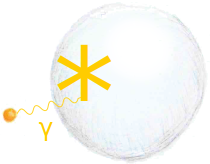
\includegraphics[height=0.3\textheight]{general/HydrogenWithPhoton.pdf}}}
%       \only<3>{\put(290,120){\includegraphics[height=0.3\textheight]{general/proton.png}}}
      \only<2>{\put(290,120){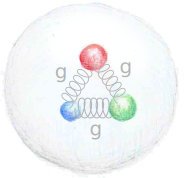
\includegraphics[height=0.3\textheight]{general/protonWithGluons.pdf}}}
      \only<1,2>{
        \put(0,68){
          \begin{minipage}{0.5\textwidth}
            \begin{itemize}\itemsep1pt
            \item \textbf{Subject:} all charged particles
            \item \textbf{Charge:} electrical charge (+, -)
            \item \textbf{Force carrier:} photon ($\gamma$)\\
            \item \textbf{Range:} $\infty$
            \item \textbf{Coupling constant:} $\alpha = \frac{e^2}{4\pi} = \frac{1}{137}$
            \item \textbf{Strength:} $\propto \frac{1}{r^2}$  
            \end{itemize}
          \end{minipage}
        }
      }
      \only<2>{
        \put(210,50){
          \begin{minipage}{0.6\textwidth}
            \begin{itemize}\itemsep1pt
            \item \textbf{Subjects:} quarks \& anti-quarks (u,d,s,c,b,t)
            \item \textbf{Charge:} color charge (r,g,b, $\bar{\text{r}}$, $\bar{\text{g}}$, $\bar{\text{b}}$,)
            \item \textbf{Force carrier:} 8 gluons (carry color charge)
            \item \textbf{Range:} $10^{-15}$ m $\approx$ nucleus size
            \item \textbf{Coupling constant:} $\alpha_s = \frac{g_s^2}{4\pi} \sim 1$
            \item \textbf{Strength:} $\propto \frac{4}{3}\frac{\alpha_s}{r} + kr$
            \item No observation of standalone quarks \\
                  confined into colorless hadrons:\\
                  Baryons (qqq) or Mesons (q$\bar{\text{q}}$)
            \end{itemize}
          \end{minipage}
        }
      }
   \end{picture}
  \end{frame}
  
  \begin{frame}{The Phase Diagram}
   \begin{picture}(340,220)
      \only<1,2>{\put(0,2){\includegraphics[height=0.84\textheight]{general/phasediagram_water.pdf}}}
      \only<3,4>{\put(0,2){\includegraphics[height=0.85\textheight]{general/phasediagram_own_v2.pdf}}}
      \only<5>{\put(0,2){\includegraphics[height=0.85\textheight]{general/phasediagram_own_withExp_v2.pdf}}}
      \only<1,2>{\put(40,210){\textbf{Phase diagram of Water}}}
      \only<3-5>{\put(40,210){\textbf{Phase diagram of QCD matter}}}
      \put(220,210){\textbf{Characterizing Matter:}}
      \put(220,195){Temperature ($T$) vs. }
      \put(320,195){Pressure ($P$)}
      \only<2-5>{
        \put(210,180){\textcolor{AliceBlue}{$\Rightarrow$} governed by QED}
      }
      \only<3-5>{
        \put(220,160){\textbf{Characterizing QCD Matter:}}
        \put(220,145){Temperature ($T$) vs. Net-Baryon Density ($\mu_B$)}
        \put(220,130){\textcolor{AliceBlue}{$\Rightarrow$} governed by QCD}
      }
      \only<4,5>{
        \put(210,105){
        \begin{minipage}{0.5\textwidth}
          \begin{itemize}
          \item Quark Gluon Plasma (QGP) created in early phase of universe
          \end{itemize}
        \end{minipage}
        }
      }
      \only<5>{
        \put(210,55){
        \begin{minipage}{0.5\textwidth}
          \begin{itemize}
          \item Study QGP created in heavy-ion collisions at particle accelerators
                \begin{itemize}
                 \item First observations at SPS \& RHIC
                 \item LHC currently most powerful accelerator \\ - pp \@ 13 TeV \& Pb--Pb \@ 5.02 TeV -
                \end{itemize}
          \item QGP world's best liquid  ($\eta/s \approx 0.08$)
          \end{itemize}
        \end{minipage}
        }
      }
   \end{picture}
  \end{frame}

  
  \begin{frame}{}
    \begin{picture}(340,220)
      \put(40,200){\textcolor{AliceBlue}{\LARGE How can we study the properties of the QGP?}}
      \put(320,20){\includegraphics[width=0.25\textwidth]{general/question.JPG}}
      \put(30,55){\includegraphics[height=0.45\textheight]{general/qpg.png}}
      \put(67,10){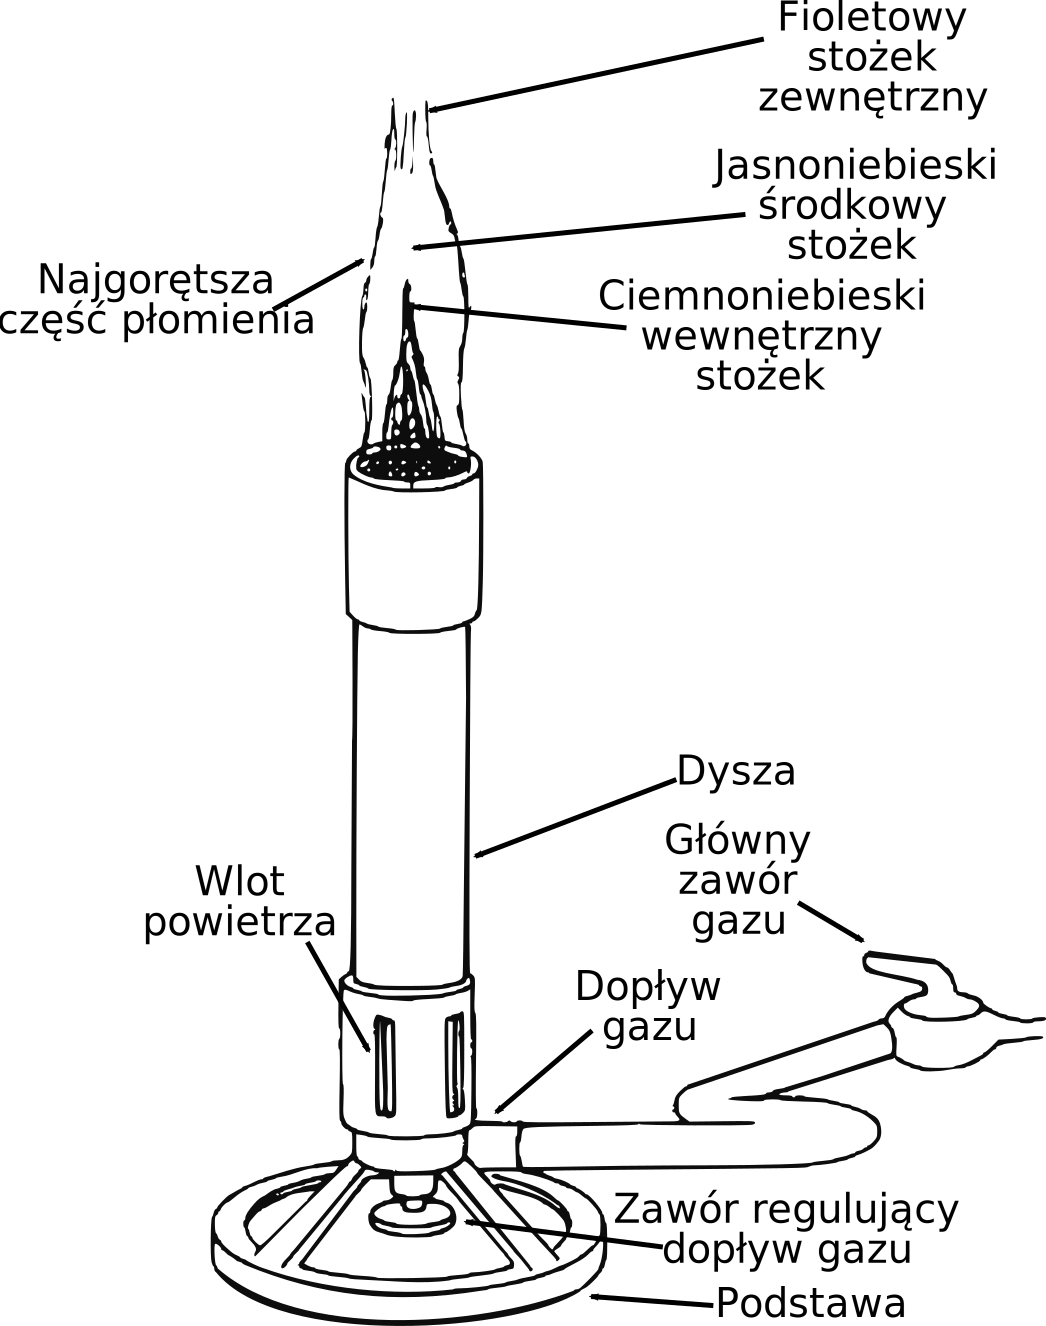
\includegraphics[height=0.2\textheight]{general/Bunsen_burner_scheme.pdf}}
      \only<2>{
        \put(155,10){\includegraphics[height=0.7\textheight]{general/qgp_dijet.eps}}
        \thicklines
        \put(22,170){\color{AliceRed2}{\line(2,-3){108}}}
        \put(22,10){\color{AliceRed2}{\line(2,3){108}}}
      }
    \end{picture}
  \end{frame}
%   /home/fbock/Photon/Presentations/
  

  \begin{frame}{Stopping Power of QED \& QCD}
   \begin{picture}(340,220)
      \only<1,2>{
        \put(-10,125){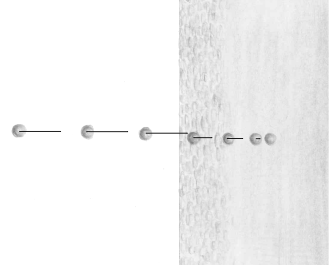
\includegraphics[width=0.23\textwidth]{general/energyLossNormalMatter.pdf}}
        \put(330,120){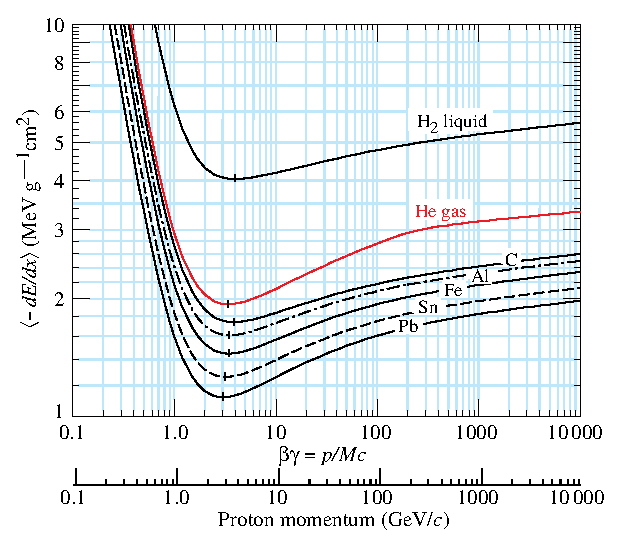
\includegraphics[width=0.25\textwidth]{OakridgeTalk/energyLossProtons.eps}}
        \put(135,210){\textcolor{AliceBlue}{\textbf{Energy loss in normal matter}}}
        \put(100,160){
          \begin{minipage}{0.5\textwidth}
            \small
            \begin{equation*}
             \hspace{-0.3cm}\Delta E = L \rho \left( K z^2 \frac{Z}{A} \frac{1}{\beta^2} \left[ \frac{1}{2} \ln{\frac{2 m_e c^2 \beta^2 \gamma^2 T_{max}}{I^2}} - \beta^2 - \frac{\delta(\beta \gamma)}{2}   \right] \right)
            \end{equation*}
            \tiny
            $A$: atomic mass of absorber, $K/A \sim 0.3$ MeV/g cm$^2$ for A = 1 g mol$^{-1}$, \\
            $z$ \& $Z$ atomic number of incident particle \& absorber, \\
            $T_{max}$ maximum transfered energy, \\
            $I$ characteristic ionization constant, \\
            $L$ length of medium
          \end{minipage}
        }
      }
      \only<2>{
        \put(-5,15){\includegraphics[width=0.23\textwidth]{general/energyLossQGP_withArrows.pdf}}
        \put(330,5){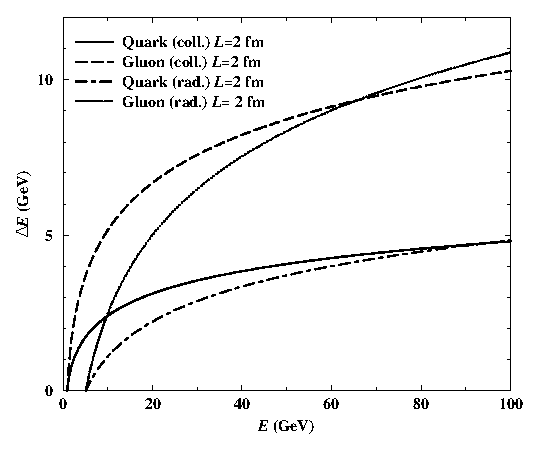
\includegraphics[width=0.25\textwidth]{OakridgeTalk/energylossQGP.eps}}
        \put(145,100){\textcolor{AliceBlue}{\textbf{Energy loss in the QGP}}}
        \put(100,60){
          \begin{minipage}{0.5\textwidth}
            \small
            \begin{equation*}
              \Delta E \propto \alpha_S C_F \hat{q} L^2, \hspace{1cm} \hat{q} = \frac{\mu^2}{\lambda}
            \end{equation*}
            \tiny 
            $C_F$ Casimir factor (3 for gluons and 4/3 for quarks),\\
            $L$ length of medium,\\
            $\mu^2$ typical momentum transfer from medium to parton per collision,\\
            $\lambda$ mean free path in medium \\
          \end{minipage}
        }
      }
    \end{picture}
  \end{frame}

  \begin{frame}{Energy Loss in the Medium}
    \begin{picture}(340,220)
        \only<1>{\put(14.5,120){\includegraphics[height=0.4\textheight]{general/qpg.png}}}
        \only<2>{\put(0,122){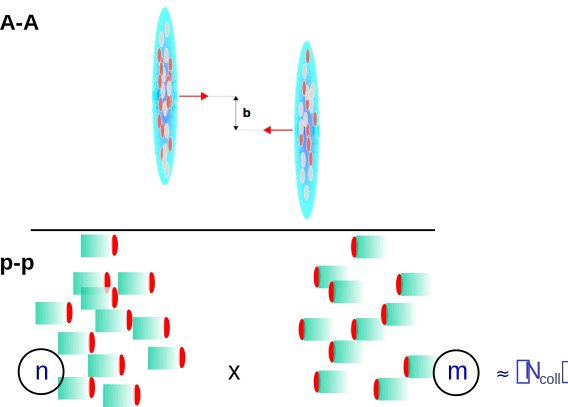
\includegraphics[width=0.3\textwidth]{EMLectureWeek2018/RAApicturePre.pdf}}}
        \only<3-6>{\put(0,120){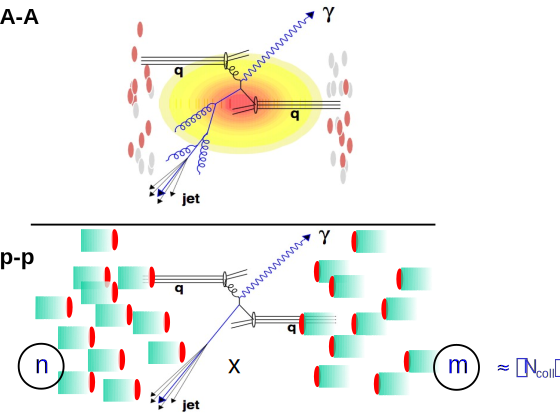
\includegraphics[width=0.3\textwidth]{EMLectureWeek2018/RAApicture.pdf}}}
%         \only<3-7>{\put(0,120){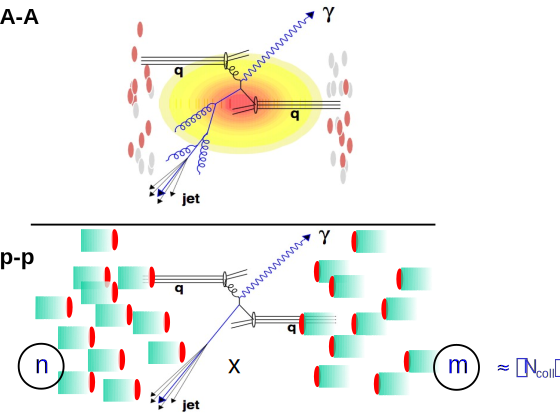
\includegraphics[width=0.3\textwidth]{EMLectureWeek2018/RAApicture.pdf}}}
        \only<4>{\put(310,5){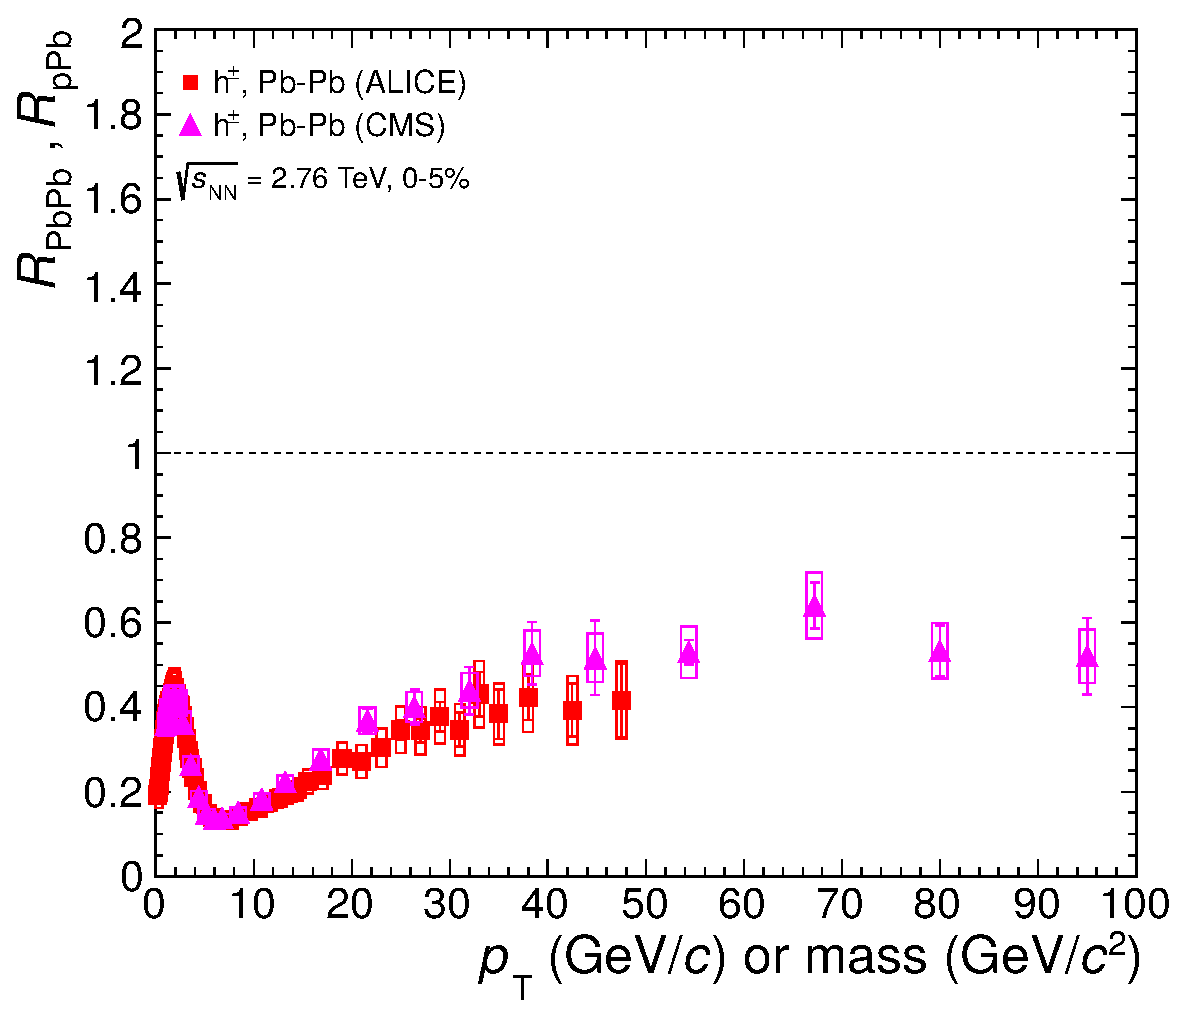
\includegraphics[width=0.3\textwidth]{OakridgeTalk/RAA_all2-5093_woControlProbes_wopPb.eps}}}
        \only<5>{\put(310,5){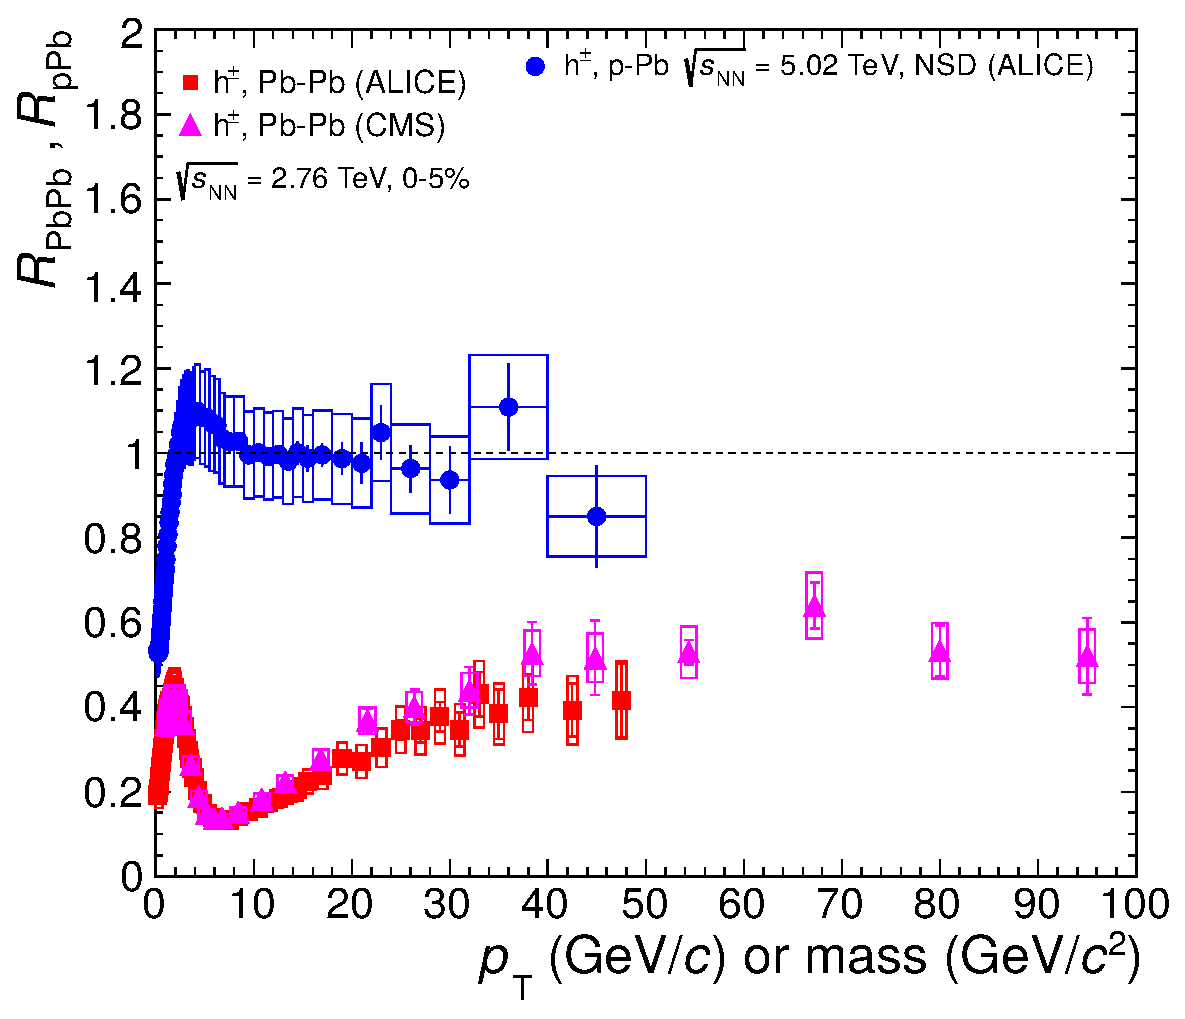
\includegraphics[width=0.3\textwidth]{OakridgeTalk/RAA_all2-5093_woControlProbes.eps}}}
        \only<6>{\put(310,5){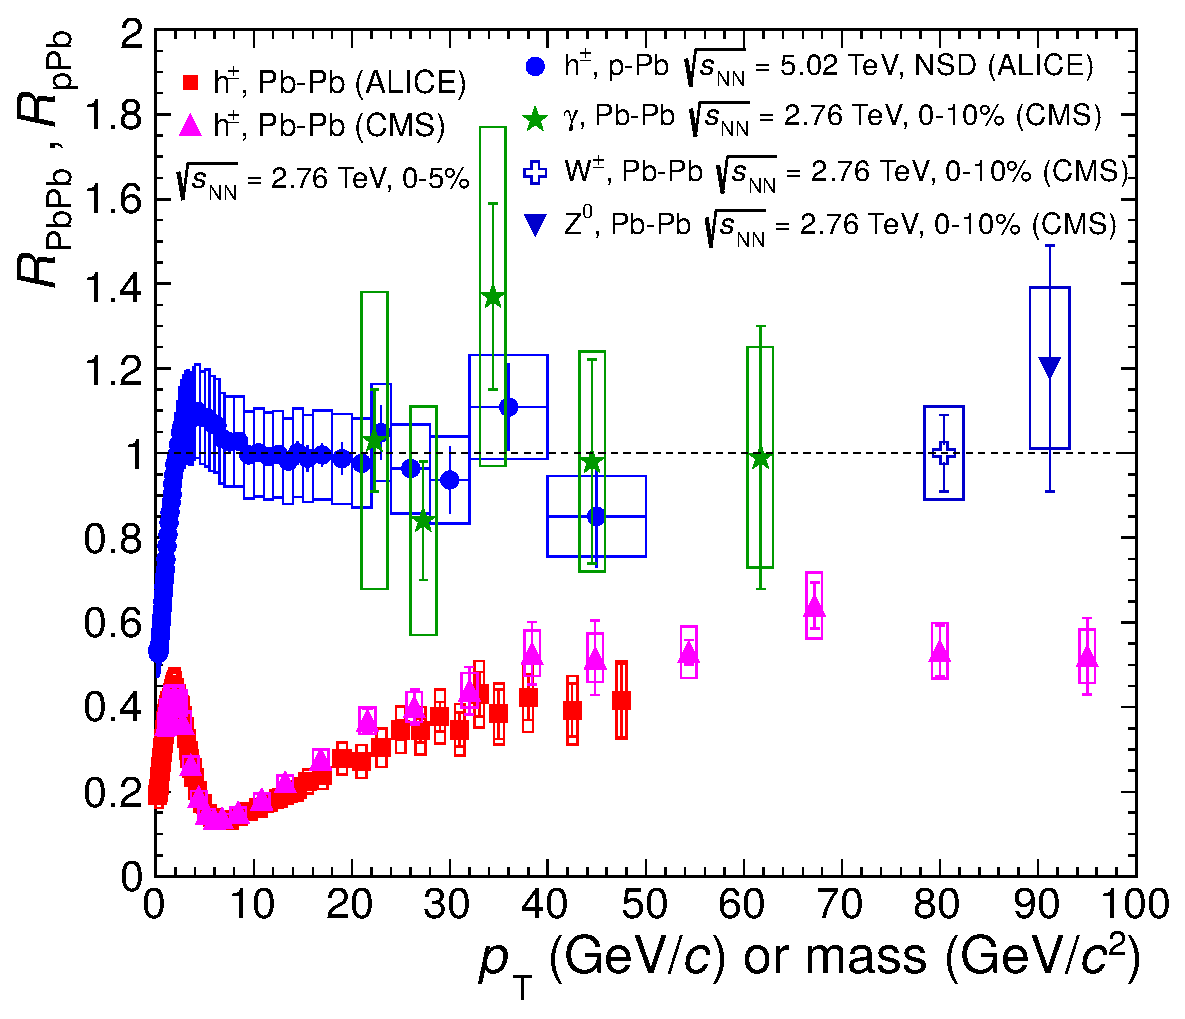
\includegraphics[width=0.3\textwidth]{OakridgeTalk/RAA_all2-5093.eps}}}
%         \only<7>{\put(310,5){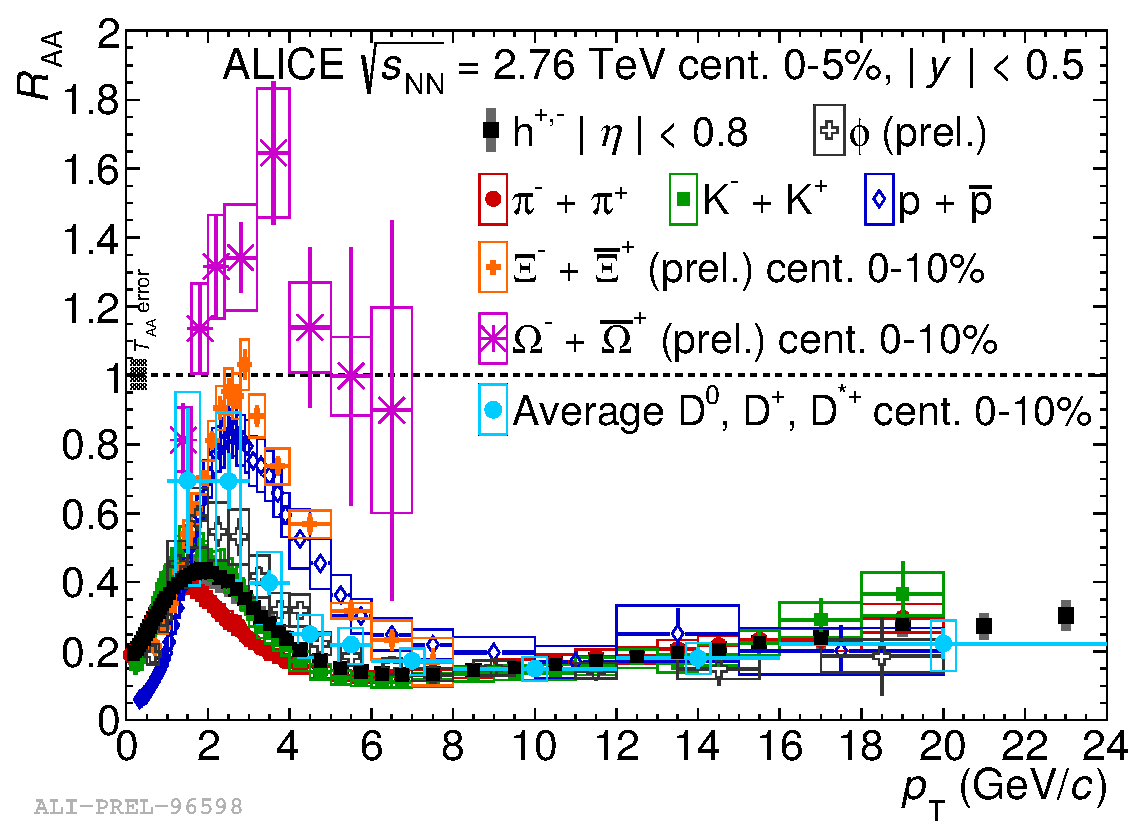
\includegraphics[width=0.3\textwidth]{OakridgeTalk/2015-Sep-16-comp_raa_LFandDmesons_cent0.eps}}}
        \put(110,212){\textbf{\textcolor{AliceBlue}{How can one interpret heavy-ion in comparison to pp collisions?}}}
        \only<2-6>{
%         \only<2-7>{
          \put(110,170){
            \begin{minipage}{0.7\textwidth}
              \begin{itemize}\itemsep0pt
                \item Can they be treated as superposition of many binary collisions of the individual protons? (binary scaling)
                \item Or are there other effects modifying these binary collisions?
              \end{itemize}
              \vspace{-0.4cm}
              \begin{eqnarray*}
%                 \RAA = \frac{\frac{1}{\NAA_{\text{\tiny evt}}} d^2\NAA/d\eta d\pT}{\langle \Ncoll\rangle \frac{1}{N_{evt}^{pp}} d^2\Npp_{\text{\tiny evt}}/d\eta d\pT}
                \RAA = \frac{d\NAA/d\pT}{\langle \Ncoll\rangle d\Npp/d\pT}
              \end{eqnarray*}            
            \end{minipage}
          }
        }
        \only<4-6>{
%         \only<4-7>{
          \put(-5,65){
            \begin{minipage}{0.4\textwidth}
              \textbf{Final state effects:}
%               Initially produced partons lose energy in medium - jet quenching:
              \begin{itemize}\itemsep0pt
              \item Parton energy loss in medium - \\jet quenching:
%               \item Scattering on other partons
%               \item [$\rightarrow$] Gluon radiation
              \item [$\rightarrow$] Depends on \textcolor{AliceBlue}{path length ($L$) in medium}
              \item [$\rightarrow$] Depends on type of parton and \textcolor{AliceBlue}{coupling strength to medium}
  %              \item Released energy can be used to create additional soft gluons \& quark-anti-quark pairs or photons
              \end{itemize}
            \end{minipage}
          }
        }
        \only<5-6>{
%         \only<5-7>{
          \put(170,78){
            \begin{minipage}{0.3\textwidth}
              \textbf{Initial state effects:}\\
              present in pA \& AA collisions
              \begin{itemize}\itemsep0pt
              \item Cronin effect
              \item Nuclear PDFs
              \item Color Glass Condensate
              \end{itemize}
            \end{minipage}
          }
        }
    \end{picture}
  \end{frame}

  \begin{frame}{Anisotropic Flow}
    \begin{picture}(340,220)
      \put(-5,140){\includegraphics[width=0.28\textwidth]{OakridgeTalk/Planck_s_view_of_the_cosmic_microwave_background.jpg}}
      \only<1,2>{\put(11.5,0){\includegraphics[height=0.5\textheight]{general/qpg.png}}}
      \only<3-4>{\put(-7,0){\includegraphics[height=0.5\textheight]{general/qgp_v2.eps}}}
      \only<3,4>{\put(320,120){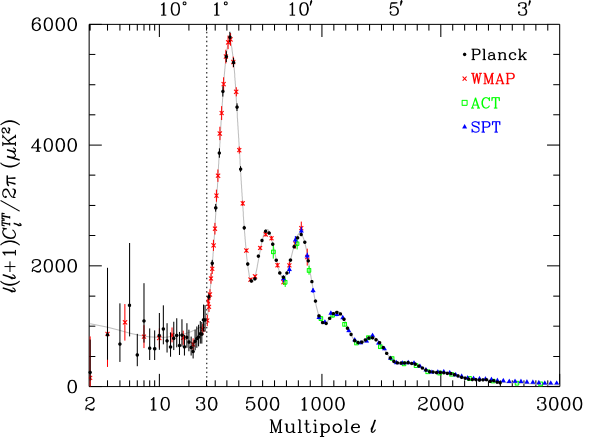
\includegraphics[width=0.28\textwidth]{OakridgeTalk/CMB_fit.pdf}}}
      \only<4>{\put(320,0){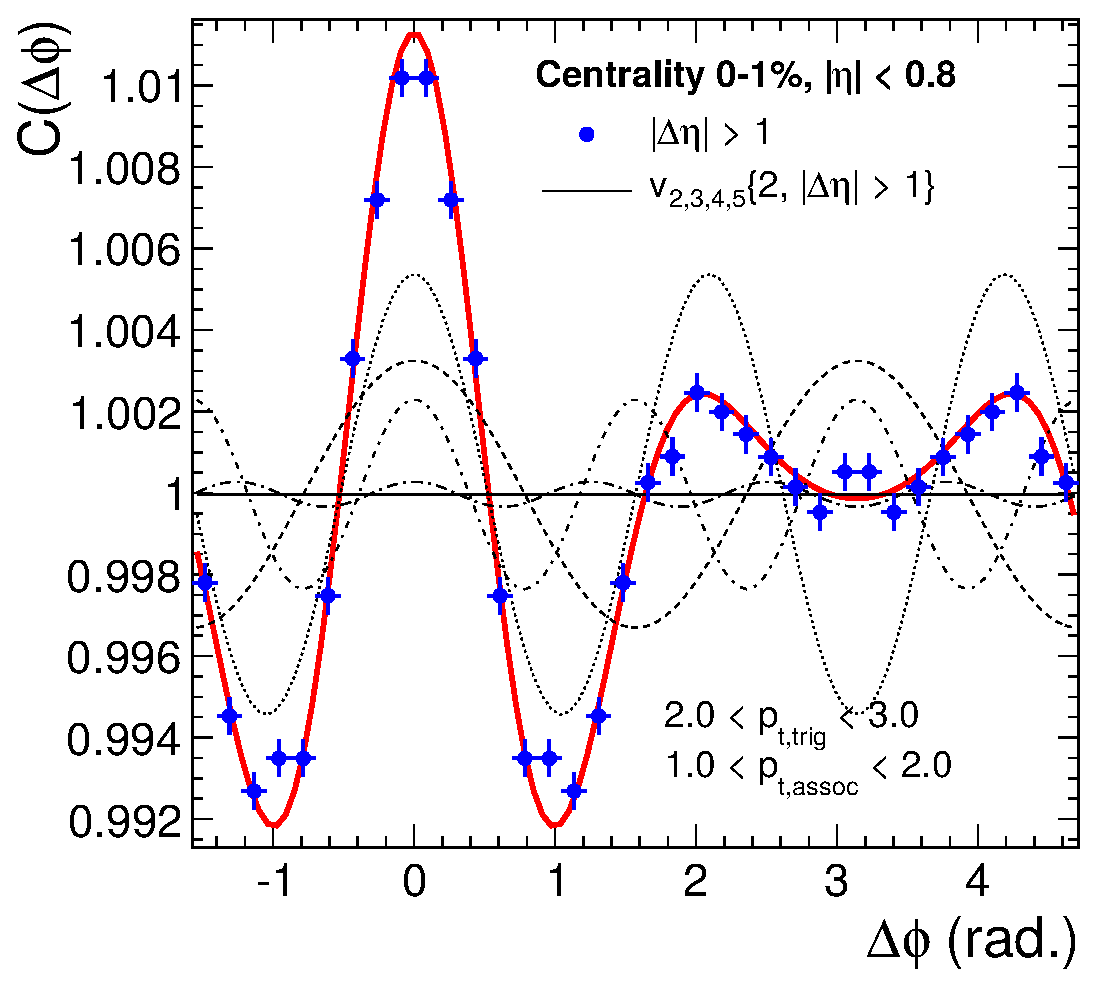
\includegraphics[width=0.28\textwidth]{OakridgeTalk/Fig4-27016.eps}}}
      \only<2-4>{
        \put(125,180){
          \begin{minipage}{0.4\linewidth}
            Initial azimuthal asymmetry in coordinate space in non-central A+A causes\\ \textcolor{AliceBlue}{initial inhomogeneities of system's energy density and pressure} \newline $\Rightarrow$ asymmetry in  momentum space
          \end{minipage}          
        }
      }
      
      \only<3-4>{  
        \put(127,135){Fourier decomposition:}
        \put(124,117){          
          \small
%           \\
          \fbox{$\frac{\mathrm{d}N}{\mathrm{d}\varphi} = \frac{1}{2\pi}\left(1+2\sum_{n\ge1}\nu_{n}\cos(n(\varphi-\Psi_n^{RP}))\right)$}
        }
      }
     \only<4>{
        \put(125,70){
          \begin{minipage}{0.4\linewidth}
            \begin{itemize}
              \item Magnitude of $\nu_n$'s depends on properties of plasma \& initial anisotropies
            \end{itemize}
          \end{minipage}
        }
     }
    \end{picture}
  \end{frame}
  
%   \begin{frame}{Viscosity of the Medium}
%     \begin{picture}(340,220)
%         \only<1>{\put(14.5,120){\includegraphics[height=0.4\textheight]{general/qpg.png}}}
%         \only<2-4>{\put(0,120){\includegraphics[height=0.4\textheight]{general/qgp_v2.eps}}}
%         \only<2>{\put(-5,5){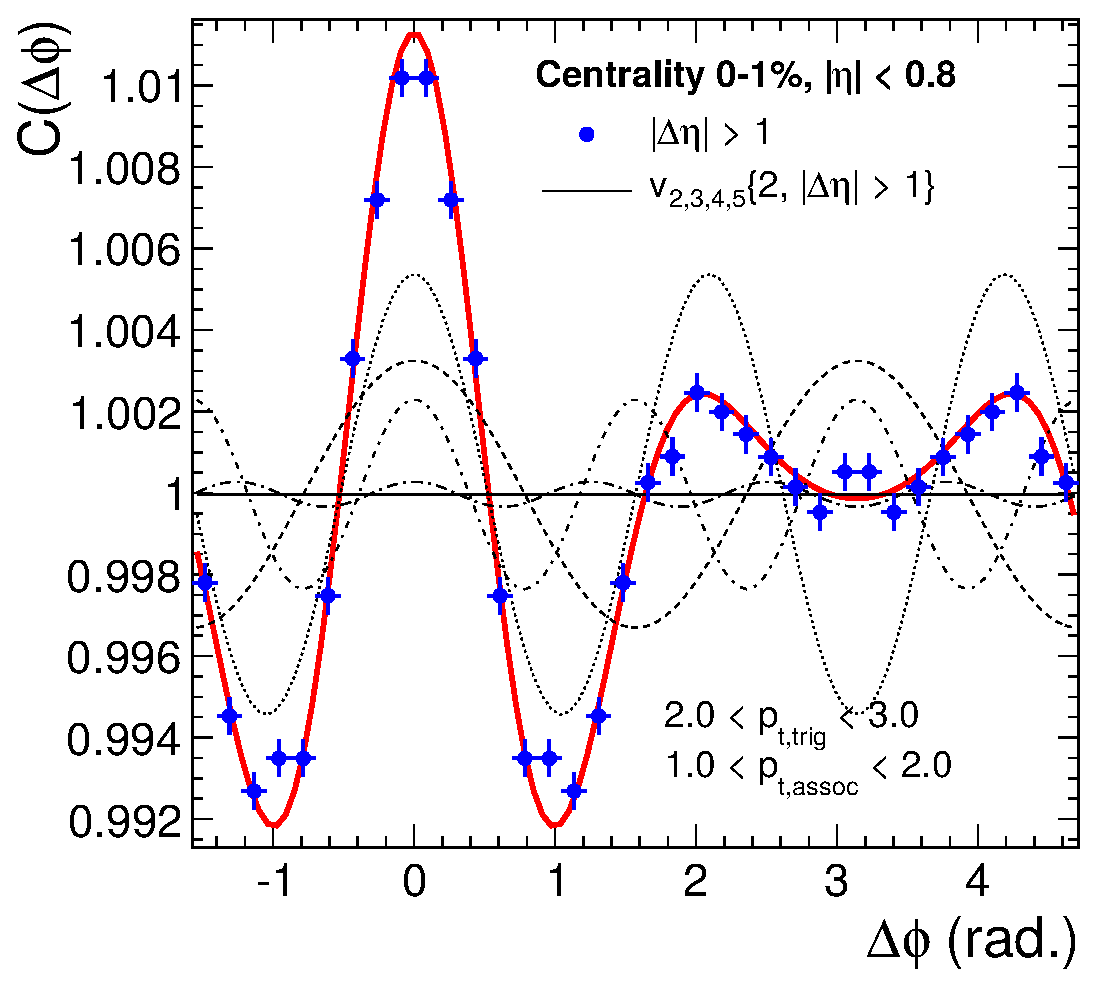
\includegraphics[height=0.42\textheight]{OakridgeTalk/Fig4-27016.eps}}}
%         \only<3>{\put(-5,5){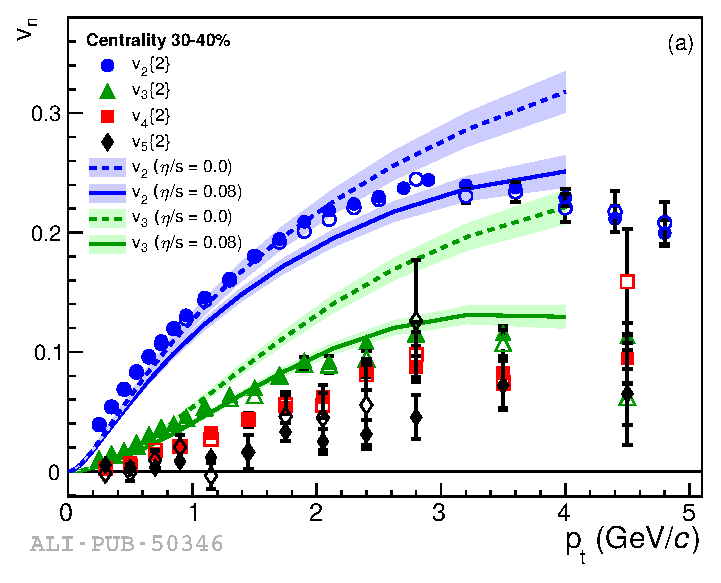
\includegraphics[height=0.42\textheight]{OakridgeTalk/2013-Jun-20-Fig3.eps}}}
%         \only<4>{\put(-5,10){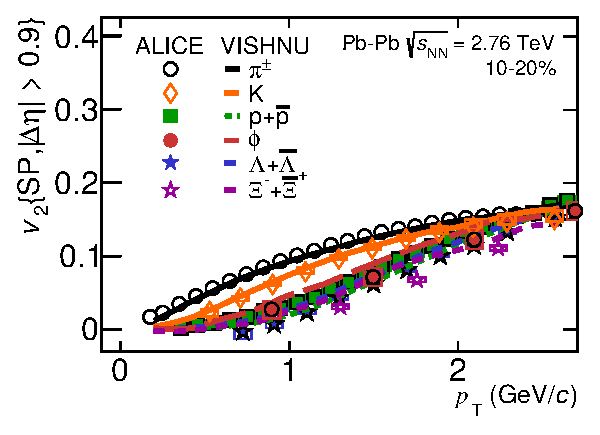
\includegraphics[height=0.38\textheight]{OakridgeTalk/v2DataVsHydroAvgK-13304.eps}}}
%         \only<2-4>{
%           \put(110,123){
%             \begin{minipage}{.75\linewidth}
%               Different harmonics of anisotropic flow sensitive to:
%               \begin{itemize}\itemsep1pt
%               \item \textcolor{AliceBlue}{Equation of state (EOS)}
%               \item \textcolor{AliceBlue}{Transport coefficients of medium} - \\shear ($\eta/s$) and bulk ($\xi/s$) viscosity to entropy density ratio
%               \end{itemize}
%             \end{minipage}
%           }
%         }
%         \only<4>{
%           \put(130,50){
%             \begin{minipage}{.67\linewidth}
%              Anisotropic flow components can constrain in addition:
%              \begin{itemize}\itemsep1pt
%               \item Initial spatial densities 
%               \item Freeze-out conditions
%               \item Particle production mechanisms in different $\pT$ regions
% %               \item Rescattering and regeneration in the hadronic phase
% %               \item Late-stage interactions
%              \end{itemize}
%              $\Rightarrow$ Study $\nu_n$ for different particle species to distinguish different effects
%             \end{minipage}
%           }
%         }
%     \end{picture}
%   \end{frame}

  
  \begin{frame}{Viscosity of the Medium}
    \begin{picture}(340,220)
%         \put(0,120){\includegraphics[height=0.4\textheight]{general/qgp_v2.eps}}
        \only<1-3>{\put(-5,115){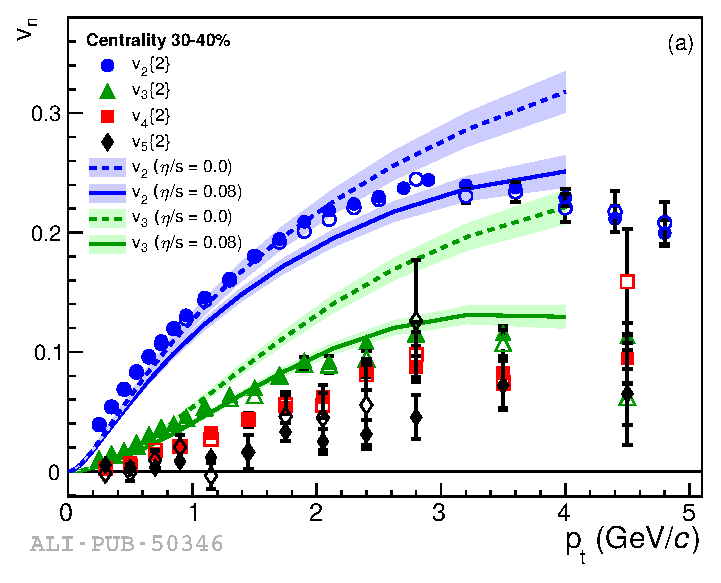
\includegraphics[height=0.42\textheight]{OakridgeTalk/2013-Jun-20-Fig3.eps}}}
        \only<3>{\put(-5,10){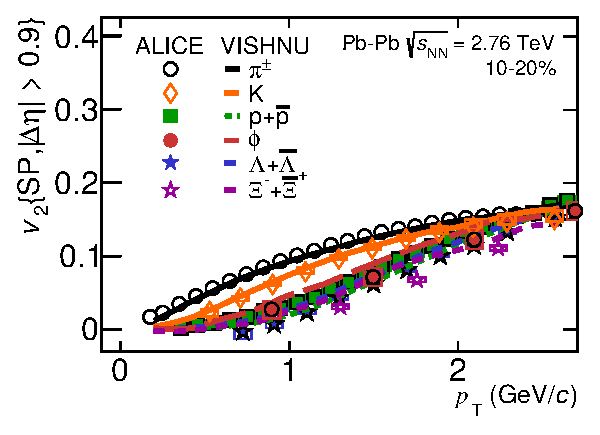
\includegraphics[height=0.38\textheight]{OakridgeTalk/v2DataVsHydroAvgK-13304.eps}}}
        \put(125,163){
          \begin{minipage}{.5\linewidth}
            Different harmonics of anisotropic flow sensitive to:
            \begin{itemize}\itemsep1pt
            \item \textcolor{AliceBlue}{Equation of state (EOS)}
            \item \textcolor{AliceBlue}{Transport coefficients of medium}:
                  \begin{itemize}
                   \item shear viscosity to entropy density ratio  \textcolor{AliceBlue}{$\eta/s$ } \\
                         $\rightarrow$ dampens buildup of $\nu_2, \nu_3, \dots$
                   \item bulk viscosity to entropy density ratio \textcolor{AliceBlue}{$\xi/s$ } \\
                        $\rightarrow$ dampens buildup of radial flow
                  \end{itemize}
            \end{itemize}
            Used in relativistic hydrodynamic calculations for the evolution of heavy ion collisions
          \end{minipage}
        }
        \only<2,3>{\put(350,118){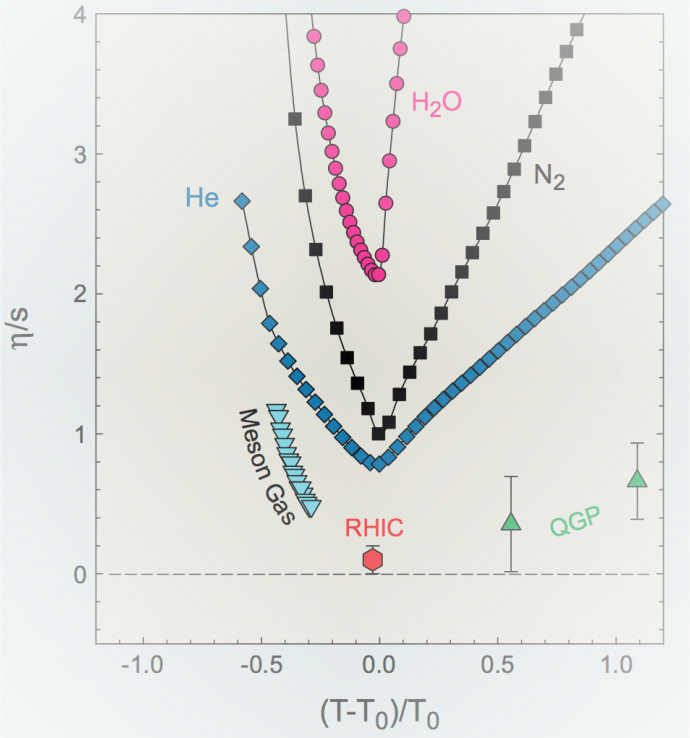
\includegraphics[width=0.21\textwidth]{OakridgeTalk/etaOverSSummary.png}}}
        
        \only<3>{
          \put(125,65){
            \begin{minipage}{.7\linewidth}
             Anisotropic flow components can constrain in addition:
             \begin{itemize}\itemsep1pt
              \item Initial spatial densities 
              \item Freeze-out conditions
              \item Particle production mechanisms in different $\pT$ regions
%               \item Rescattering and regeneration in the hadronic phase
%               \item Late-stage interactions
             \end{itemize}
             $\Rightarrow$ Study $\nu_n$ for different particle species to distinguish different effects
            \end{minipage}
          }
        }
    \end{picture}
  \end{frame}
  
  \begin{frame}{Temperature of the Medium}
    \begin{picture}(340,220)
        \put(280,118){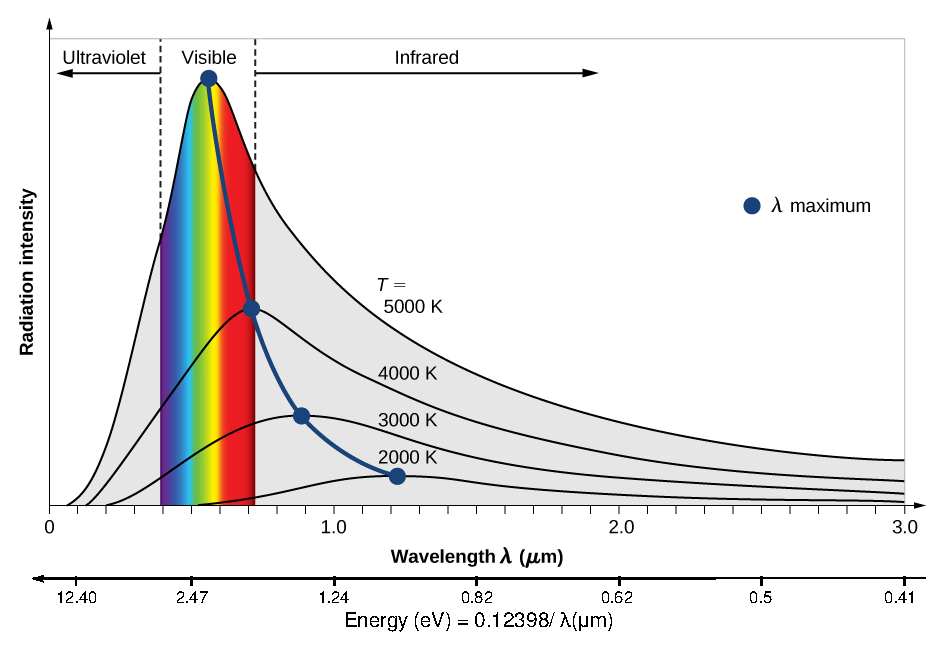
\includegraphics[width=0.35\textwidth]{general/blackbodyRad.eps}}
%         \only<1>{\put(14.5,10){\includegraphics[height=0.4\textheight]{general/qpg.png}}}
%         https://phys.libretexts.org/Bookshelves/University_Physics/Book%3A_University_Physics_(OpenStax)/Map%3A_University_Physics_III_-_Optics_and_Modern_Physics_(OpenStax)/6%3A_Photons_and_Matter_Waves/6.1%3A_Blackbody_Radiation
        \only<2,3>{\put(0,20){\includegraphics[height=0.4\textheight]{general/qgp_thermal.eps}}}
        \only<3>{\put(290,5){\includegraphics[width=0.34\textwidth]{general/v2_photon.pdf}}}
        \put(0,200){\begin{minipage}{.6\linewidth} \textbf{\textcolor{AliceBlue}{Expected temperature (up to $\approx 10^{12}$ K) \\ $\mathbf{\approx 10^5~\times~T_{\text{\tiny core sun}} \approx 2.5 \cdot 10^8~\times~T_{\text{\tiny photoshere sun}}}$ }} \end{minipage}}
        \put(10,170){\textbf{Stefan's law}}
        \put(0,150){
          \fbox{$P(T) = \sigma A T^4$}
        }
        \put(110,170){\textbf{Planck's blackbody radiation law}}
        \put(130,150){
          \fbox{$I(\lambda, T) = \frac{2\pi hc^2}{\lambda^5}\frac{1}{e^{hc/\lambda k_B T}-1}$}
        }
        \only<2,3>{
          \put(90,70){
            \begin{minipage}{0.5\linewidth}
              \textcolor{AliceBlue}{Measure photons emitted by QGP over \\full energy spectrum }
              \begin{itemize}
                \item Directly related to temperature of plasma
                \item Expansion of plasma $\Rightarrow$ cooling \& further photon emission
                \item [$\Rightarrow$] measured $T$ $\equiv$ blue shifted $T_{eff}$
                \item Need to know at which time photons are produced
              \end{itemize}
            \end{minipage}
          }
        }
        
    \end{picture}   
  \end{frame}

  \section{Direct Photons}
  \begin{frame}{}
    \begin{picture}(340,220)
      \put(5,200){\textcolor{AliceBlue}{\LARGE What makes direct photon measurements so difficult?}}
      \put(380,145){\includegraphics[width=0.15\textwidth]{general/question.JPG}}
      \only<1>{
        \put(80,40){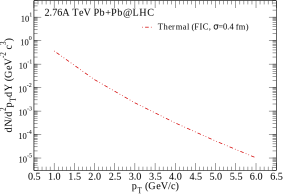
\includegraphics[width=0.5\textwidth]{general/theroryOnlyCurves_buildUp.pdf}}
      }
      \only<2>{
        \put(80,40){\includegraphics[width=0.5\textwidth]{general/theroryOnlyCurves.pdf}}
      }
      \only<3,4>{
        \put(80,40){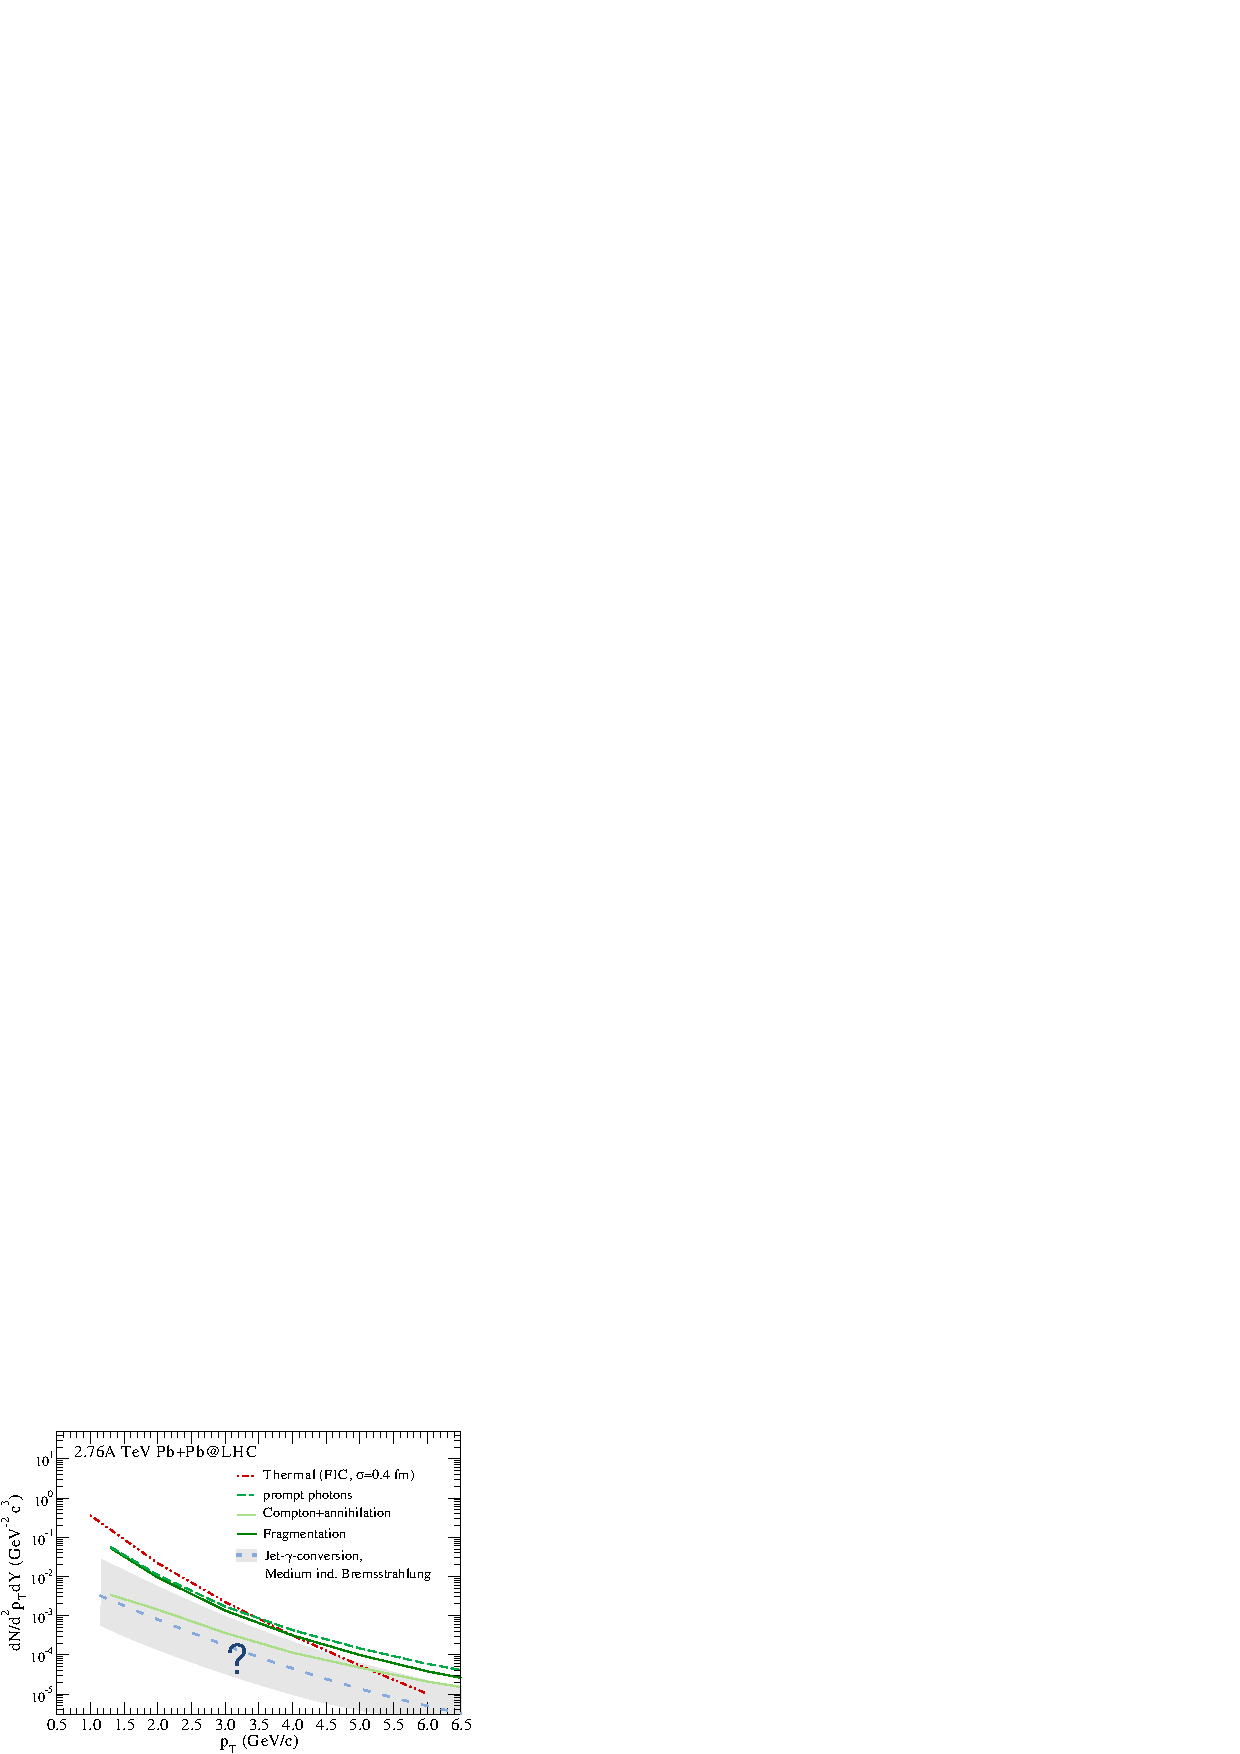
\includegraphics[width=0.5\textwidth]{general/theroryOnlyCurves_buildUp3.pdf}}
      }
      \put(0,70){\includegraphics[width=0.15\textwidth]{general/qgp_thermal.eps}}
      \only<2-4>{
        \put(310,-5){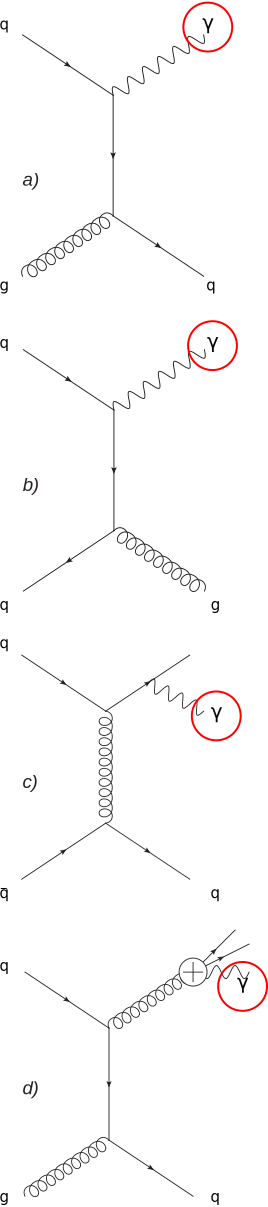
\includegraphics[width=0.10\textwidth]{general/feymangraphs_vertical.pdf}}
        \put(370,70){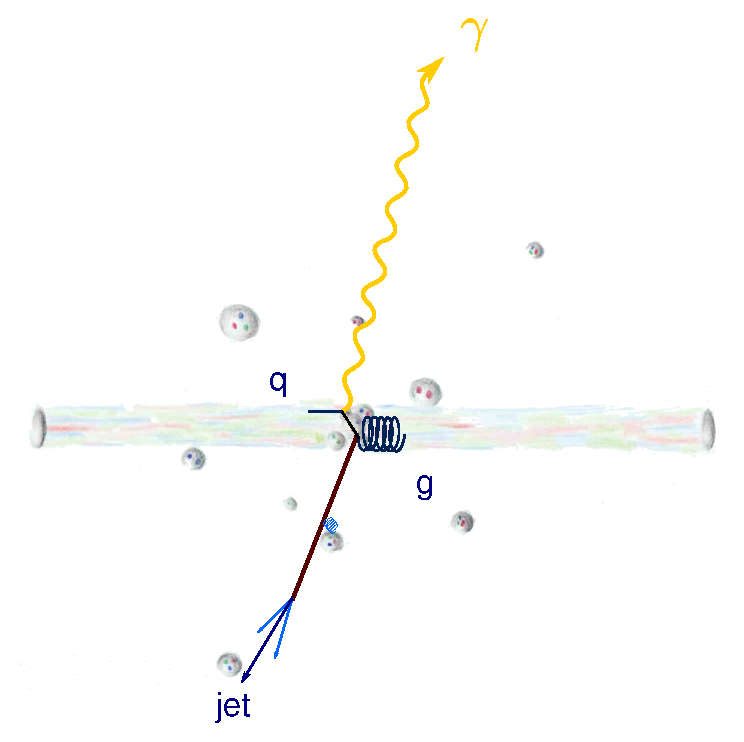
\includegraphics[width=0.15\textwidth]{general/pp_photonJet.eps}}
        \put(380,50){\textcolor{AliceGreen}{\textbf{\large pp $\times \mathbf{\Ncoll}$}}}
      }
      \only<3,4>{
        \put(120,-12){\includegraphics[width=0.10\textwidth]{general/qgp_photonbremstrahlung.eps}}
        \put(220,-12){\includegraphics[width=0.10\textwidth]{general/qgp_photonJet.eps}}      
      }
      \only<4>{
        \put(0,10){\textbf{\large $\mathbf{\gamma_{\text{\tiny dir}}}$ only 10-20\%}}
        \put(0,-5){\textbf{\large of detectable $\mathbb{\gamma}$}}
      }
    \end{picture}
  \end{frame}
%   
%   \begin{frame}{Challenges of Direct Photon Measurements}
%     \begin{columns}
%       \begin{column}{9.5cm}
%         \vspace{-1.55cm}
%         \begin{itemize}\itemsep3pt
%         \item Large background from decay photons\\
%               nearly all neutral light mesons decay partially in $\gamma$: $\pi^0, \eta, \omega, \eta', \phi \ldots$
%         \item Experimentally not easy to distinguish decay photons from $\pi^0(\eta)$ with small opening angle from single photons as they merge into one detector signal
%         \item Small impurities in inclusive photon measurement can lead to large effects in direct photon measurement
%         \end{itemize}
%       \end{column}
%       \begin{column}{4.8cm}

%       \end{column}
%     \end{columns}
%     \vspace{-1.35cm}
%     \begin{columns}
%         \begin{column}{4.8cm}
%           \includegraphics[width=\textwidth]{EMLectureWeek2018/DR_Theory_pPb5TeV.pdf}
%         \end{column}
%         \begin{column}{10cm}
%           \vspace{1cm}
%           \begin{itemize}\itemsep3pt
%           \item Expected direct photon signals in pp \& p--A collisions 1-3\% at low $\pT$ and even in A--A collisions only $\sim 20\%$
%           \item Finding isolated photons in large background in A--A or p-A collisions
%           \end{itemize}
%         \end{column}
%     \end{columns}
%   \end{frame}

  \begin{frame}{Direct Photon Extraction}
    \begin{picture}(340,220)
      \put(-5,160){
        \begin{minipage}{0.75\textwidth}
          \underline{\textbf{Subtraction Method}}:
          \vspace{-0.2cm}
            \begin{eqnarray*}
            \gamma_{\text{direct}} &=& \gamma_{\text{inclusive}}-\gamma_{\text{decay}} = (1-\frac{\textcolor{AliceGreen}{\gamma_{\text{decay}}}}{\textcolor{AliceRed}{\gamma_{\text{inclusive}}}})\cdot\gamma_{\text{inc}}\\ \vspace{-1cm}
                  &=& (1-\frac{1}{R_{\gamma}})\cdot\gamma_{\text{inclusive}}
            \end{eqnarray*}
          \vspace{-0.5cm}
          \begin{itemize}
          \item Inclusive photons: measure all photons that are produced
          \item Decay photons: calculated from measured particle spectra with photon decay branches ($\pi^0$, $\eta$, ...) by a particle decay (cocktail) calculation
          \end{itemize}
        \end{minipage}
      }
      \put(320,96){\includegraphics[width=0.275\textwidth]{EMLectureWeek2018/pPbDirGammaPrelim/2018-May-04-CocktailGammasRatioToAll_0_80_80000113_00200009327000008250400000_0162103500000000.pdf}}
      \only<2>{
        \put(-5,55){
          \begin{minipage}{0.7\textwidth}
            \flushleft
            \underline{\textbf{Double Ratio}}:\\
            \center
            $R_{\gamma} = \textcolor{AliceRed}{\frac{\gamma_{\text{inclusive}}}{\pi^{0}}} / \textcolor{AliceGreen}{\frac{\gamma_{\text{decay}}}{\pi^{0}_{\text{param}}}} \approxeq \frac{ \textcolor{AliceRed}{\gamma_{\text{inclusive}}}}{ \textcolor{AliceGreen}{\gamma_{\text{decay}}}}$\hspace{0.5cm} if $> 1$ direct photon signal\\
            \flushleft $\rightarrow$ advantage of double ratio method: cancellation of uncertainties
            \begin{itemize}
            \item \textcolor{AliceRed}{Numerator}: Inclusive $\gamma$ spectrum per $\pi^0$
            \item \textcolor{AliceGreen}{Denominator}: Sum of all decay photons per $\pi^0$
            \end{itemize}
          \end{minipage}
        }
        \put(323,4){\includegraphics[width=0.268\textwidth]{EMLectureWeek2018/DR_Theory_pPb5TeV.pdf}}
      }
    \end{picture}
  \end{frame}


  \begin{frame}{Measuring Photons, $\pi^0$ and $\eta$ Mesons with ALICE}
    \begin{picture}(340,220)
    
      \only<1>{\put(-10,0){\includegraphics[height=0.91\textheight]{general/ALICEdetectorLayoutReducedLabeling_elong.pdf}}}
      \only<1>{
        \put(0,30){\textbf{ALICE collaboration}}
        \put(0,20){177 institutes from 41 countries}
        \put(0,10){$\approx$ 1800 members}
        \put(335,210){19 sub-detector systems}
        \put(360,200){weight: $\sim$10000 t}
        \put(362,190){height: $\sim$16 m}
        \put(362,180){length: $\sim$26 m}
        
      }
      \only<2-3>{\put(80,3){\includegraphics[height=0.9\textheight]{HP2018/event102_cropped_blueish3.png}}}
      \only<3>{\put(20,3){\includegraphics[width=0.30\textwidth]{QM2018/pPbMesonsPaper/2018-Mar-07-Pi0_MassAndWidth_incPHOSandDalitz.pdf}}}
%       \only<3>{\put(5,142){\tiny arXiv:1801.07051}}
      \only<2-3>{
        \put(275,180){
          \begin{minipage}{0.49\linewidth}
            \textbf{Photon Conversion Method (PCM)}
            \begin{itemize}
              \item ITS and TPC
              \item $|\eta| < 0.9, ~0^{\circ} < \varphi < 360^{\circ}$ 
              \item conversion in detector material
                    \begin{itemize}
                    \item $X/X_{0} = (11.4\pm0.5)\%$
                    \item conv. probability $\sim 8\%$
                    \end{itemize}
            \end{itemize}
          \end{minipage}
        }
        \put(300,40){
          \begin{minipage}{0.30\linewidth}
          \textbf{PHOS calorimeter}
          \begin{itemize}
            \item PbWO$_{4}$ crystals
            \item $|\eta| < 0.12$ ,\\ $260^{\circ} < \varphi < 320^{\circ}$ \tiny (2009-2013) 
          \end{itemize}
          \end{minipage}
        }
        \put(-10,170){
          \begin{minipage}{0.49\linewidth}
          \textbf{EMCal calorimeter}
          \begin{itemize}
            \item Pb/scintillator \\sampling calorimeter
            \item $|\eta| < 0.7$,\\ $80^{\circ} < \varphi < 180^{\circ}$ 
            \item Designed \& built \\
                  by ORNL
          \end{itemize}
          \end{minipage}
        }
      }
    \end{picture}
  \end{frame}
  
  \begin{frame}{}
    \begin{picture}(340,220)
      \put(0,200){\textcolor{AliceBlue}{\Huge What have we learned so far from}}
      \put(25,170){\textcolor{AliceBlue}{\Huge direct photon spectra measurements?}}
      \put(320,10){\includegraphics[width=0.3\textwidth]{general/flashlight.png}}
      \put(-5,-15){\includegraphics[width=0.22\textwidth]{general/pp_photonJet.eps}}
      \put(95,20){\includegraphics[width=0.22\textwidth]{general/pA_photonJetMidRapidity.pdf}}
      \put(200,70){\includegraphics[width=0.22\textwidth]{general/pA_withQGP_thermal.pdf}}
      \put(150,-10){\textcolor{AliceBlue}{\Large Small systems: pp \& p-Pb}}
    \end{picture}
  \end{frame}

  
    \begin{frame}{Direct Photons in pp}
    \begin{picture}(340,220)
      \only<1>{
        \put(20,86){\includegraphics[width=0.38\textwidth]{HP2018/pp_DirGamma/2018-Mar-27-DR_CombAndTheory_pp2760GeV_NonFit.pdf}}
        \put(235,86){\includegraphics[width=0.38\textwidth]{HP2018/pp_DirGamma/2018-Mar-27-DR_CombAndTheory_NonFit_pp8TeV.pdf}}
%         \put(300,103){\includegraphics[width=0.266\textwidth]{HP2018/pp_LMll/pp_r_pythia-30612.eps}}
%         \put(376,216.5){\tiny arXiv:1805.04391}
      }
      \put(144,216.5){\tiny arXiv:1803.09857}
      \put(359,216.5){\tiny arXiv:1803.09857}
      
      \put(-20,43){
        \begin{minipage}{0.52\linewidth}
        \begin{itemize}
         \small
         \itemsep0.5em  
          \item Systematic uncertainties of individual meas.\\% $\approx 5-8\%$ at $\pT < 4$ GeV/$c$\\
                $\rightarrow$ dominated by $\pT$-independent\\
                  material unc. of 4.5\% PCM \& 2.8\% EMC \\
          \item $\pT$ reach
            \begin{itemize}
             \itemsep0.0em  
             \item $0.4 < \pT < 10$ GeV/$c$ in pp, $\sqrt{s} = 2.76$ TeV
             \item $0.3 < \pT < 14$ GeV/$c$ in pp, $\sqrt{s} = 8$ TeV
            \end{itemize}
          
%           \item <2> NLO prediction plotted as \\ \hspace{0.6cm}$R_{\text{\tiny NLO}} = 1+ (\gamma_{\text{\tiny dir}}^{\text{\tiny NLO}} \cdot N_{\text{Coll}})/\gamma_{\text{\tiny dec}}$
        \end{itemize}
        \end{minipage}
      }
      \only<1>{
      \put(205,43){
        \begin{minipage}{0.52\linewidth}
        \begin{itemize}
          \small
         \itemsep0.7em  
          \item Combination of 3 reconstruction techniques 
          \item \textcolor{AliceBlue}{Within uncertainties no significant excess at low $\pT$ observed}\\
          \item [$\rightarrow$] supports interpretation in Pb--Pb as medium effects
          \item About $1-2\sigma$ deviation from unity for $\pT > 7$ GeV/$c$
%           \item \textcolor{AliceBlue}{All pp results at the LHC with similar uncertainties }
        \end{itemize}
        \end{minipage}
      }
      }
    \end{picture}
  \end{frame}

  \begin{frame}{Direct Photons in p--Pb at low \pT}
  \begin{picture}(340,220)
    \put(-20,120){
      \begin{minipage}{0.4\linewidth}
        \begin{itemize}
          \itemsep0.7em
          \item Combination of 4 reconstruction techniques
          \item Individual sys uncertainties O(5-10\%), combined total O(4-5\%)
          \item Upper limits at 90\% C.L. (arrows) determined where $R_{\gamma}$ with total uncertainties consistent with unity
          \item <2> \textcolor{AliceBlue}{0-20\% central collisions don't show a significant excess}
          \item <2> \textcolor{AliceBlue}{NLO \& thermal \textit{\tiny (Shen et al.)} calculations consistent with measurements }
        \end{itemize}
      \end{minipage}
    }
    \only<1>{
      \put(159,124){\includegraphics[width=0.27\textwidth]{HP2018/p-A_DirGamma/2018-May-07-DRNonFit_IndMeasurements_pPb5TeV.pdf}}
      \put(159,30){\includegraphics[width=0.27\textwidth]{HP2018/p-A_DirGamma/2018-May-06-DRNonFit_CombAndTheory_pPb5TeV.pdf}}
      \put(277,25){\includegraphics[width=0.39\textwidth]{HP2018/p-A_DirGamma/2018-May-04-InvYield_DirGamma_IncGamma_Theory.pdf}}
    }
    \only<2>{
      \put(159,124){\includegraphics[width=0.27\textwidth]{HP2018/p-A_DirGamma/2018-09-28-DR_IndMeasurements_pPb5TeV_00-20.pdf}}
      \put(159,30){\includegraphics[width=0.27\textwidth]{HP2018/p-A_DirGamma/2018-09-28-DR_CombAndTheory_pPb5TeV_00-20.eps}}
      \put(277,25){\includegraphics[width=0.39\textwidth]{HP2018/p-A_DirGamma/InvYield_DirGamma_IncGamma_Theory_00-20.pdf}}
    }
    \put(0,20){Theory calculations from: }
    \put(0,10){\small W. Vogelsang \tiny{(CT10,nCTEQ15,EPPS16/GRV)}, \small J.F. Paquet \tiny{(CTEQ6.1M/BFG)}, \small C. Shen \tiny{}}
%     \put(385,10){\tiny \href{https://indico.cern.ch/event/656452/contributions/2869645/attachments/1648426/2635388/QM2018_v2.pdf}{Friederike Bock, QM 2018}}
    \put(379,5){\tiny Shen \textit{et al.} arXiv:1609.02590}
  \end{picture}
  \end{frame}

  \begin{frame}{}
    \begin{picture}(340,220)
      \put(0,200){\textcolor{AliceBlue}{\Huge What have we learned so far from}}
      \put(25,170){\textcolor{AliceBlue}{\Huge direct photon spectra measurements}}
      \put(50,140){\textcolor{AliceBlue}{\Huge at low and intermediate $p_{\text{\normalsize T}}$?}}
      \put(320,10){\includegraphics[width=0.3\textwidth]{general/flashlight.png}}
      \put(20,-10){\includegraphics[width=0.25\textwidth]{general/qgp_thermal.eps}}
      \put(170,-10){\textcolor{AliceBlue}{\Large Large Systems: A-A}}
    \end{picture}
  \end{frame}

  \begin{frame}{Direct Photons in Pb-Pb}
    \begin{picture}(340,220)
      \put(226,5){\only<2>{\includegraphics[width=7.6cm]{EMLectureWeek2018/PbPbDirGammaPaper/2015-Sep-24-DR_combMeasurement_incNLO.pdf}}}
      \put(226,5){\only<1>{\includegraphics[width=7.6cm]{EMLectureWeek2018/ppDIrGammaPaper/2018-Mar-26-DR_PbPbWithRefPP.pdf}}}
%       \put(286,125){\only<3>{\includegraphics[width=5cm]{EMLectureWeek2018/PbPbDirGammaPaper/2015-Sep-24-DirGammaRAA_0020.pdf}}}
%       \put(286,10){\only<3>{\includegraphics[width=5cm]{EMLectureWeek2018/PbPbDirGammaPaper/2015-Sep-24-DirGammaRAA_2040.pdf}}}
%       \put(226,5){\only<4>{\includegraphics[width=7.6cm]{EMLectureWeek2018/ppDIrGammaPaper/2018-Mar-26-DirGammaSpectra_WithScaledPP_Split.pdf}}}
      \only<2>{\put(270,6){\tiny PLB 754 (2016) 23-248}}
      \only<1>{\put(270,6){\tiny \href{https://cdsweb.cern.ch/record/2310535/files/Public\%20Note.pdf}{ALICE-PUBLIC-2018-001}}}
%       \only<3>{\put(300,6){\tiny \href{https://cdsweb.cern.ch/record/2102398/files/public_note.pdf}{ALICE-PUBLIC-2015-007}}}
      \put(-10,115){
        \begin{minipage}{0.5\linewidth}
        \begin{itemize}
          \itemsep0.5em
          \item Direct photon excess measured with combined PCM + PHOS in 3 centrality classes with 2010 Pb–Pb data
          \item $R_{\gamma}$ excess at high $\pT$ for all centralities
          \item $\gamma^{\text{dec}}$ suppressed by $\approx \RAA^{\pi^0}$ \\$\rightarrow$ larger excess in central collisions
          \item Low $\pT\ \sim 15\%$ excess in $0-20\%$ central and\\ $\sim 9\%$ in $20-40\%$ semi central
          \item In agreement with NLO pQCD, JETPHOX above $5$ GeV/$c$
          \item No low $\pT$ excess seen in pp collisions at same center-of-mass energy
          \item Scaled pp spectrum \& upper limits fully consistent with Pb--Pb results
        \end{itemize}
        \end{minipage}
      }
    \end{picture}
  \end{frame}

  \begin{frame}{}
    \begin{picture}(340,220)
      \put(0,200){\textcolor{AliceBlue}{\Huge Which new insights did the direct photon}}
      \put(80,170){\textcolor{AliceBlue}{\Huge flow measurements reveal?}}
      \put(0,0){\includegraphics[width=0.4\textwidth]{general/v2_photon.pdf}}
      \put(320,10){\includegraphics[width=0.3\textwidth]{general/flashlight.png}}
      \put(205,110){\underline{Direct photon $\nu_{2}$:}}
      \put(193,80){\fbox{$\nu_{2}^{\gamma\text{,dir}} = \frac{R_\gamma \cdot \nu_{2}^{\gamma\text{,inc}}-\nu_{2}^{\gamma\text{,dec} } }{R_\gamma-1}$}}
      \put(170,40){
        \begin{minipage}{0.4\textwidth}
          \begin{itemize}
            \item Small $\nu_{2}$ $\rightarrow$ early emission
            \item Large $\nu_{2}$ $\rightarrow$ late emission
          \end{itemize}
        \end{minipage}
      }
    \end{picture}
  \end{frame}

\frame{
  \frametitle{Direct Photon Yield and Flow - At the LHC}
  \begin{picture}(340,220)
%     \put(290,83){\includegraphics[width=0.33\textwidth]<2>{EMLectureWeek2018/PbPbDirGammaFlowPaper/2040_v2dir_combined_theory.eps}}
%     \put(145,57){\includegraphics[width=0.33\textwidth]<2>{EMLectureWeek2018/PbPbDirGammaFlowPaper/020_v2dir_combined_theory.eps}}
    \put(290,83){\only<2>{\includegraphics[width=0.33\textwidth]{EMLectureWeek2018/PbPbDirGammaFlowPaper/2018-May-11-2040_v2dir_combined_theory.pdf}}}
    \put(145,61){\only<2>{\includegraphics[width=0.33\textwidth]{EMLectureWeek2018/PbPbDirGammaFlowPaper/2018-May-11-020_v2dir_combined_theory.pdf}}}
    \put(-8,4){\includegraphics[width=0.33\textwidth]{EMLectureWeek2018/PbPbDirGammaPaper/2015-Sep-24-DirGammaSpectrumPlusMcGill_ReducedX.pdf}}
    \put(81,169){\tiny PLB 754 (2016) 23-248}
    \only<2>{\put(249,201){\tiny arXiv:1805.04403}}
    \put(-15,199){
      \begin{minipage}{0.68\linewidth}
        \begin{itemize}
          \item Central points for direct photon yield and $\nu_{2}^{\gamma\text{,dir}}$ underestimated by most theoretical calculations \\
                by factors of 2-5
        \end{itemize}
      \end{minipage}
    }
    \only<2>{
      \put(130,30){
        \begin{minipage}{0.69\linewidth}
          \begin{itemize}
            \small
            \itemsep0.1em
            \item $\nu_{2}^{\gamma\text{,dir}}$ comparable to charged hadron $\nu_2$ 
            \item Mild tension between theory $\&$ experiment
            \item $\nu_{2}^{\gamma\text{,dir}}$ compatible with $\nu_{2}^{\gamma\text{,dir}}=0$ within $1.4 (1.0) \sigma$ in $\pT$ range ($0.9<\pT<2.1$ GeV/$c$)
            
%             \item No deviation beyond $2\sigma$ from theory observed for spectra or $\nu_{2}$
%             \item Similar observations for all theoretical calculations despite very different setups
          \end{itemize}
        \end{minipage}
      }
    }
  \end{picture}
}

\frame{
  \frametitle{Direct Photon Yield and Flow - Comparison to PHENIX}
  \begin{picture}(340,220)
    \put(290,83){\includegraphics[width=0.33\textwidth]{EMLectureWeek2018/PbPbDirGammaFlowPaper/2018-May-11-2040_v2dir_combined_phenix.pdf}}
    \put(145,83){\includegraphics[width=0.33\textwidth]{EMLectureWeek2018/PbPbDirGammaFlowPaper/2018-May-11-020_v2dir_combined_phenix.pdf}}    
%     \put(290,83){\includegraphics[width=0.33\textwidth]{EMLectureWeek2018/PbPbDirGammaFlowPaper/2040_v2dir_combined_phenix.eps}}
%     \put(145,83){\includegraphics[width=0.33\textwidth]{EMLectureWeek2018/PbPbDirGammaFlowPaper/020_v2dir_combined_phenix.eps}}
    \put(-8,4){\only<1>{\includegraphics[width=0.33\textwidth]{EMLectureWeek2018/PbPbDirGammaPaper/2015-Sep-25-DirGammaSpectrumPlusPHENIX0020_ReducedX.pdf}}}
    \put(-8,4){\only<2>{\includegraphics[width=0.33\textwidth]{EMLectureWeek2018/PbPbDirGammaPaper/2015-Sep-25-DirGammaSpectrumPlusPHENIX2040_ReducedX.pdf}}}
    \put(81,169){\tiny PLB 754 (2016) 23-248}
    \put(161,88){\tiny arXiv:1805.04403}
    \put(-15,193){
      \begin{minipage}{0.35\linewidth}
        \begin{itemize}\itemsep0pt
          \item Photon yield increased by\\ $\approx$ factor 2 for $\pT\ < 3$ GeV/$c$
          \item Larger $T_{\text{eff}}$ for direct photons at the LHC energies  
        \end{itemize}
      \end{minipage}
    }
    \put(150,40){
      \begin{minipage}{0.6\linewidth}
        \begin{itemize}
          \item $\nu_{2}$ compatible with $\nu_{2}$ measured at $\sqrt{s_{_{NN}}} = 0.2$ TeV
          \item Similar scaling behavior of direct photon $\nu_{2}$ as for charged hadrons
          \item Larger significance for PHENIX result due to larger $R_{\gamma}$ and larger significance of $R_{\gamma}$ at $\sqrt{s_{_{NN}}} = 0.2$ TeV
        \end{itemize}
      \end{minipage}
    }
  
    \end{picture}
  }
  \section{Future Instrumentation Opportunities}
  
  \begin{frame}{}
    \begin{picture}(340,220)
      \put(10,200){\textcolor{AliceBlue}{\Huge How can we improve our understanding}}
      \put(0,170){\textcolor{AliceBlue}{\Huge of the QGP and hadron collisions in general?}}
      \put(360,60){\includegraphics[width=0.18\textwidth]{general/question.JPG}}
      \put(0,100){\includegraphics[width=0.2\textwidth]{general/ppCollisions.png}}
      \put(95,60){\includegraphics[width=0.2\textwidth]{general/pACollisions_woQGP.png}}
      \put(185,20){\includegraphics[width=0.2\textwidth]{general/pACollisions_QGP.png}}
      \put(275,-18){\includegraphics[width=0.2\textwidth]{general/qpg.png}}
      \put(100,140){\textbf{\large pp}}
      \put(200,120){\textbf{\large p-Pb}}
      \put(300,100){\textbf{\large Pb-Pb}}
%       \put(10,0){\textbf{\large Future Instrumentation}}
    \end{picture}
  \end{frame}

  \begin{frame}{Exploring the Pre-equilibrium State of Heavy Ion Collisions}
    \begin{picture}(340,220)
      \put(0,146){\includegraphics[width=0.24\textwidth]{OakridgeTalk/2018-Jul-23-New_Pre_V2_CC2030_gap08_hydro.pdf}}
      \put(0,3){\includegraphics[width=0.24\textwidth]{OakridgeTalk/2018-Jul-23-New_Pre_newv3v4_v3v4_gap08_hydro.pdf}}
      \only<2,3,4>{\put(300,62){\includegraphics[width=0.25\textwidth]{general/IPGlasma.pdf}}}
      \only<2,3,4>{\put(330,-6){\includegraphics[width=0.25\textwidth]{general/MCGlauber.pdf}}}
      \put(300,140){\includegraphics[width=0.31\textwidth]{general/glasma_lightcone.pdf}}
      \put(110,140){
        \begin{minipage}{0.44\linewidth}
          \begin{itemize}\itemsep5pt
           \item Description of data by hydrodynamic calculations not only dependent on transport properties of QGP
           \item <2,3,4>Detailed understanding of initial conditions and pre-equilibrium state essential
           \item <3,4>Signals of collective behavior of similar size as in peripheral A-A collisions also seen in smaller systems (high mult p-A and pp)\\
          \end{itemize}\vspace{0.3cm}
        \end{minipage}
      }
      \only<4>{\put(110,40){\begin{minipage}{0.49\linewidth}\centering \textbf{\textcolor{AliceBlue}{Can part of the final state effects\\  be explained by modifications of the \\
      nuclear parton distribution functions (nPDFs)? }}\end{minipage} }}
    \end{picture}
  \end{frame}

  \begin{frame}{Understanding the Proton and Ion Substructure}
    \begin{picture}(340,220)
      \put(-8,113){\includegraphics[width=0.28\textwidth]{general/CGCIllustration.eps}}
      \only<2-5>{\put(-8,5){\includegraphics[width=0.26\textwidth]{OakridgeTalk/focal-EMprobesCoverage_onlyDIS.pdf}}}
      \only<6>{\put(-8,5){\includegraphics[width=0.26\textwidth]{OakridgeTalk/focal-EMprobesCoverage_woFOCAL_woEIC.pdf}}}
%       \only<7>{\put(-8,5){\includegraphics[width=0.26\textwidth]{OakridgeTalk/focal-EMprobesCoverage_woFOCAL.pdf}}}
%       \only<8>{\put(-8,5){\includegraphics[width=0.26\textwidth]{OakridgeTalk/focal-EMprobesCoverage.pdf}}}
      \only<3>{\put(364,113){\includegraphics[height=0.44\textheight]{OakridgeTalk/nPDFQ1000_builtUp.pdf}}}
      \only<1-3>{\put(364,5){\includegraphics[height=0.44\textheight]{OakridgeTalk/nPDFQ10_buildUp.pdf}}}
      \only<4-6>{\put(364,113){\includegraphics[height=0.44\textheight]{OakridgeTalk/nPDFQ1000.pdf}}}
      \only<4-6>{\put(364,5){\includegraphics[height=0.44\textheight]{OakridgeTalk/nPDFQ10.pdf}}}
      \put(110,113){
        \begin{minipage}{0.55\linewidth}
          \begin{itemize}
%            \small
          \item Largest fraction of energy in proton ($x$) carried by 3 valence quarks (2u,d)
          \item <2-6> Experimentally measured in electron-proton collisions \tiny{(Deep Inelastic Scattering (DIS)})
          \item <3-6> Increasing the transfered momentum (Q) does not change picture drastically, calculable in QCD
          \item <4-6> At low $x$ large contribution from gluons \& sea-quarks
          \item <4-6> Gluon density cannot grow indefinitely at low x \\$\Rightarrow$ onset of nonlinear behavior of soft color fields\\ \hspace{0.25cm} above $Q_{\text{\tiny S}}$ necessary\\
                    $\Rightarrow$ \textcolor{AliceBlue}{Gluon Saturation}
          \item <5-6> Evolution of PDFs along $x$ axis not calculable in QCD\\
          \item <5-6> Effective theory for low $x$-\\
                \textcolor{AliceBlue}{Color Glass Condensate (CGC)}
          \end{itemize}
        \end{minipage}
      }
%       \only<6-8>{\put(115,20){\begin{minipage}{0.55\linewidth} \centering \textbf{\textcolor{AliceBlue}{Can we measure the saturation effects at the current or future facilities?}}\end{minipage}}}                                                                                                                                                                        
    \end{picture}
  \end{frame}

  \begin{frame}{Future Measurements of Gluon Saturation Region}
    \begin{picture}(340,220)
      \only<1,2>{\put(-8,115){\includegraphics[width=0.26\textwidth]{OakridgeTalk/focal-EMprobesCoverage_woFOCAL.pdf}}}
      \only<1,2>{\put(354,120){\includegraphics[height=0.41\textheight]{OakridgeTalk/LongRangePlanCover.png}}}
      \only<1,2>{\put(-8,25){\includegraphics[width=0.26\textwidth]{general/eic_diagram.pdf}}}
      \only<1,2>{\put(40,10){\textcolor{AliceBlue}{EIC}}}
      
      \only<2>{\put(-8,115){\includegraphics[width=0.26\textwidth]{OakridgeTalk/focal-EMprobesCoverage.pdf}}}
      \only<2>{\put(364,25){\includegraphics[height=0.34\textheight]{general/feymann_gluonQark_photonquark.pdf}}}
      \only<2>{\put(388,10){\textcolor{AliceBlue}{FoCal}}}
      \put(110,193){
        \begin{minipage}{0.52\linewidth}
          \small
          \textbf{2015 Long Range Plan for Nuclear Science}\\
          \textit{``We recommend a high-energy high-luminosity polarized EIC as the highest priority for new facility construction following the completion of FRIB.''}
        \end{minipage}
      }
      \put(105,145){
        \begin{minipage}{0.55\linewidth}
          \begin{itemize}\itemsep0pt
            \small
            \item \textcolor{AliceBlue}{\textbf{Electron-Ion Collider (EIC)}} will explore a new QCD frontier of ultra-dense gluon fields
            \item Potential to \textcolor{AliceBlue}{discover a new form of gluon matter} predicted to be common to all nuclei
          \end{itemize}
        \end{minipage}
      }
      \only<2>{
        \put(110,100){
          \begin{minipage}{0.54\linewidth}
            \small
            \textcolor{AliceBlue}{ \textbf{Forward calorimetry in ALICE} to study gluon density distributions inside nuclei at ultra small-x well before the EIC}
          \end{minipage}
        }
        \put(105,45 ){
          \begin{minipage}{0.55\linewidth}
            \small
            \begin{itemize}\itemsep0pt
              \item Addresses questions related to the initial state in unique phase space (earlier than EIC)
              \item Well aligned with NP-DOE program
              \item Secures strong ALICE-USA leadership into Run-4 with complete exploitation of the LHC nuclear physics program till 2029 and provides a pathway to EIC $>$ 2030
            \end{itemize}
          \end{minipage}
        }
      }
      
      
    \end{picture}
  \end{frame}

  
  \begin{frame}{FoCal in ALICE}
    \begin{picture}(340,220)
      \put(-10,68){\includegraphics[width=0.5\textwidth]{OakridgeTalk/focalLayout.png}}
      \put(200,120){
        \begin{minipage}{0.54\textwidth}
          \textbf{\textcolor{AliceBlue}{Main proposal:}}
          \begin{itemize}
          \item Forward Electromagnetic calorimeter for \textcolor{AliceBlue}{$\pi^0$} and \textcolor{AliceBlue}{$\gamma$} measurements in ALICE
          \item Position: $Z \approx 7$m (outside solenoid magnet) 
          \item Coverage: $3.3 < \eta < 5.3$
          \item \textcolor{AliceBlue}{Main challenge}: 
                \begin{itemize}
                 \item Separation $\gamma/\pi^0$ at high energy \\
                      \footnotesize{$\gamma\gamma$ separation for $\pi^0$ decay ($\pT = 10 $GeV$/c, y = 4.5, \alpha=0.5$) is $d=2$mm}
                 \item needs small Moli\`ere radius \& high granularity read-out\\
                      Si-W calorimeter with effective granularity $\approx 1$ mm$^2$
                \end{itemize}
          \item Installation: Long Shutdown 3 (2023-2025)
          \end{itemize}
          \textbf{Ideal extension:} 
          \begin{itemize}
           \item Additional hadronic calorimeter for direct photon \textcolor{AliceBlue}{isolation} and \textcolor{AliceBlue}{full jet} reconstruction \\
          \end{itemize}
        \end{minipage}
      }
      \put(40,5){\includegraphics[width=0.28\textwidth]{OakridgeTalk/FocalDesign_transverse.pdf}}
%       \put(290,10){Total estimated cost: 10-15 Mio \$ }
    \end{picture}
  \end{frame}

  
  \begin{frame}{Direct Photon Performance with FoCal}
    \vspace{-0.3cm}
    \begin{figure}
      \centering
      \includegraphics[width=0.35\textwidth]{OakridgeTalk/2018-09-26-gamma_unc_INCnlo_sqrts88_4eta5.eps}\hspace{1cm}
      \includegraphics[width=0.35\textwidth]{OakridgeTalk/2018-11-23-2018-11-23-dir_gamma_unc_8TeV8_RpPb_wEPPS16.eps}
    \end{figure}
    \vspace{-0.3cm}
    \begin{itemize}
     \item Reduction of $\pi^0$ contamination with $\approx$ factor 10
           \begin{itemize}
            \item Needs combined rejection (inv. mass, shower shape, isolation)
            \item Requires high granularity
           \end{itemize}
      \item Expected uncertainty $< 20\%$ at \pT $\sim 4$ GeV/$c$  decreasing with increasing \pT
      \item Impact: Improvement in PDF uncertainties by $\sim$ factor 2
    \end{itemize}
  \end{frame}

  \begin{frame}{Additional FoCal Physics Topics}
    \begin{figure}
      \includegraphics[width=0.33\textwidth]{OakridgeTalk/pi0pi0-corr-focal.pdf}\hspace{0.2cm}
      \includegraphics[width=0.315\textwidth]{OakridgeTalk/jetResol_focal.pdf}\hspace{0.2cm}
      \includegraphics[width=0.31\textwidth]{OakridgeTalk/PbPb_signal_exa_8pt10.pdf}
    \end{figure}
    \begin{columns}
      \begin{column}{5.2cm}
        Low-x gluons (n)PDF, saturation
        \begin{itemize}
        \item Direct photon $R_{pA}$
        \item $\pi^0\pi^0$ correlations
        \item Di-jet correlations
        \end{itemize}
        \vspace{0.2cm}
      \end{column}
      \begin{column}{7.cm}
        Ridge/flow-like phenomena in pp, p-A, A-A
        \begin{itemize}
        \item Correlations: forward photon- mid rapidity hadron (photon)
        \item Instrumentation: reaction plane determination in A-A
        \end{itemize}
       
      \end{column}
      \begin{column}{4cm}
        Jet quenching at large y
        \begin{itemize}
        \item Neutral pion $\RAA$
        \end{itemize}
       \vspace{1.2cm}
      \end{column}
   \end{columns}
  \end{frame}

  \begin{frame}{Towards a Bright Future}
    \begin{picture}(340,220)
      \put(100,170){
        \begin{minipage}{0.73\textwidth}
          \textbf{Summary of $\gamma_{\text{dir}}$ production at mid-rapidity and near time prospects:}
          \begin{itemize}\itemsep4pt
            \item Direct photons st low \pT\ in A-A collisions give access to\\
                  temperature profile of heavy-ion collisions
            \item Needs excellent understanding of photon production also in \\
                  small systems (pp \& p-A) to disentangle \\ final \& initial state signatures
          \end{itemize}
          
        \end{minipage}
      }
      \put(0,60){
        \begin{minipage}{0.65\textwidth}
          \textbf{$\gamma_{\text{dir}}$ production at forward rapidity and pathway to the EIC:} 
          \begin{itemize}\itemsep4pt
            \item Unique coverage for direct photons of proposed \\
            upgrade to ALICE FoCal to discover dense gluonic matter
            \item Allows to study the initial state and improve nPDFs significantly
            \item Future Electron-Ion Collider (EIC) to probe dense gluonic matter in detail
          \end{itemize}
        \end{minipage}
      }
      \put(0,110){\includegraphics[width=0.2\textwidth]{general/qgp_thermal.eps}}
      \put(310,20){\includegraphics[width=0.27\textwidth]{general/pA_photonJetForwardRapidity.pdf}}
    \end{picture}

  
    \begin{columns}
      \begin{column}{11.5cm}
          
      \end{column}
      \begin{column}{4.cm}
       \includegraphics[width=\textwidth]{general/idea.pdf}
      \end{column}
    \end{columns}
  \end{frame}
 
 \ifbackup
  
\frame{
  \begin{center}
    \huge{\textcolor{AliceBlue}{Backup Slides}}
  \end{center}
}

  \begin{frame}{Energy Loss in the Medium using High $\pT$ Probes}
    \begin{picture}(340,220)
        \only<1>{\put(0,120){\includegraphics[height=0.4\textheight]{general/qpg.png}}}
%         \only<2>{\put(14.5,120){\includegraphics[height=0.4\textheight]{general/qgp_gluonJet.eps}}}
        \only<2,3>{\put(0,120){\includegraphics[height=0.4\textheight]{general/qgp_dijet.eps}}}
        \only<3>{\put(0,10){\includegraphics[height=0.4\textheight]{general/qgp_photonJet.eps}}}
        \only<2,3>{\put(320,90){\includegraphics[width=0.27\textwidth]{OakridgeTalk/2015-Mar-31-fig_RAAR02Bias5CompareToHadrons.eps}}}
        \only<3>{\put(325,5){\includegraphics[width=0.27\textwidth]{OakridgeTalk/figaux_03b.pdf}}}
        \put(85,212){\textbf{\textcolor{AliceBlue}{Can we access the medium response using high $\mathbf{\pT}$ probes more directly?}}}
        \only<2,3>{
          \put(85,150){
            \begin{minipage}{0.55\textwidth}
              \textbf{Jet measurements in heavy-ion collisions}
              \begin{itemize}
              \item Jets as proxy for partons \\$\Rightarrow$ less influence of fragmentation functions
              \item Different jet radii and differential jet observables \\$\Rightarrow$ Where does the energy go?
              \item Flavor dependent jet measurements \\$\Rightarrow$ Are all partons affected in the same way?
              \end{itemize}
            \end{minipage}
          }
        }
        \only<3>{
          \put(85,50){
            \begin{minipage}{0.55\textwidth}
              \textbf{$\gamma$-Jet measurements in heavy-ion collisions}
              \begin{itemize}
              \item $\gamma$ as calibration probe for jet energy\\
                    $\Rightarrow$ How does the energy loss depend on $L$ ?
              \item $\gamma$ as tagger for predominantly quark jets and their substructure\\
                    $\Rightarrow$ Access to medium response for quark jets only?
              \end{itemize}

            \end{minipage}
          }
        }
    \end{picture}
  \end{frame}


  \begin{frame}{Definition of Direct Photons}
    \begin{columns}
     \begin{column}{1.3cm}
     \end{column}
     \begin{column}{9.7cm}        
        \textcolor{AliceBlue}{\textbf{\Large What are direct photons?}}
        \begin{itemize}
        \item [Opinion a)] Photons not coming from decays\\
        \item [$\rightarrow$] \textcolor{AliceBlue}{Experimentalist} view focussing on low momenta/energies
        \item [Opinion b)] Photons are produced without any particles in their vicinity (isolated)\\
        \item [$\rightarrow$] \textcolor{AliceBlue}{Experimentalist} view focussing on high momenta/energies
        \item [Opinion c)] Photons that are created directly in a hard scattering process\\
        \item [$\rightarrow$] Possible view of a \textcolor{AliceBlue}{theorist}
        \end{itemize}      
      \end{column}
      \begin{column}{5cm}
        \includegraphics[width=\textwidth]{general/flashlight.png}
      \end{column}
    \end{columns}
    \vspace{0.5cm}
    \centering
    \textcolor{AliceBlue}{\textbf{\Large Definition heavyly depends on physics object you want to investigate. }}
  \end{frame}

  \begin{frame}{Production Mechanisms}
    \large
   \begin{columns}
    \begin{column}{5.5cm}
     \includegraphics[width=\textwidth]{general/feymangraphs.pdf}
    \end{column}
    \begin{column}{9cm}
      \begin{itemize}
       \itemsep0.5em
       \item \textbf{Different production processes in hard scatterings}
              \begin{itemize}
              \item [a)] Quark-gluon Compton scattering
              \item [b)] Quark-quark annihilation
              \item [c)] Quark Bremsstrahlung
              \item [d)] Jet fragmentation
              \end{itemize}
        \item In the 1970's photons used to observe point like charged particles within hadrons
        \item Stringent test of QCD for high $\pT$, usually well described, ``easy" to calculate to higher orders
        \item Current focus: Constrain gluon distributions via q-g-Compton scattering at leading order
      \end{itemize}
    \end{column}
   \end{columns}
  \end{frame}

  \begin{frame}{Photon Sources in A--A and p(d)-A Collisions}
   \begin{picture}(340,220)
    \thicklines
    \only<2-6>{\put(0,5){\includegraphics[height=0.17\textheight]{general/feymangraphs_horizontal.pdf}}}
    \only<3>{\put(170,5){\includegraphics[height=0.3\textheight]{general/qgp_thermal.eps}}}
    \only<3>{\put(260,5){\includegraphics[height=0.3\textheight]{general/qgp_photonJet.eps}}}
    \only<3>{\put(350,5){\includegraphics[height=0.3\textheight]{general/qgp_photonbremstrahlung.eps}}}

    \only<5,6>{\put(200,5){\includegraphics[height=0.2\textheight]{general/qgp_thermal.eps}}}
    \only<6>{\put(305,5){\includegraphics[height=0.2\textheight]{general/qgp_photonJet.eps}}}
    \only<6>{\put(385,5){\includegraphics[height=0.2\textheight]{general/qgp_photonbremstrahlung.eps}}}
    % first classification line
    \put(143,228){\color{gray}{\line(1,0){155}}}
    \put(220,228){\color{gray}{\vector(-2,-1){40}}}
    \put(143,198){\large \textbf{Direct Photons}}
    \put(220,228){\color{gray}{\vector(4,-1){85}}}
    \put(283,198){\large \textbf{Decay Photons}}
    % second classification line
    \only<2-6>{\put(163,196){\color{gray}{\vector(-4,-1){120}}}    }
    \only<2>{\put(5,155){\color{AliceGreen}{\large \textbf{Prompt Photons}}}}
    \only<3-6>{\put(5,155){\large \textbf{Prompt Photons}}}
    \only<3-6>{
      \put(175,196){\color{gray}{\vector(-1,-2){15}}}
      \put(192,196){\color{gray}{\vector(2,-1){63}}}
      \put(220,196){\color{gray}{\vector(4,-1){120}}}

      \only<3,5,6>{ \put(110,155){\large \textbf{Pre-equilibrium}}
                \put(125,145){\large \textbf{Photons}}
               }
      \only<4>{ \put(110,155){\color{AliceYellow}{\large \textbf{Pre-equilibrium}}}
                \put(125,145){\color{AliceYellow}{\large \textbf{Photons}}}
               }
      \only<3,4,6>{ \put(210,155){\large \textbf{Thermal Photons}}}
      \only<5>{ \put(210,155){\color{AliceRed}{\large \textbf{Thermal Photons}}}}
      \only<3,4,5>{
        \put(330,155){\large \textbf{Hard + Thermal}}
        \put(350,145){\large \textbf{Photons}}
      }
      \only<6>{
        \put(330,155){\color{AliceBlue}{\large \textbf{Hard + Thermal}}}
        \put(350,145){\color{AliceBlue}{\large \textbf{Photons}}}
      }
    }
    % second classification line
    \only<2-6>{
      \put(48,153){\color{gray}{\vector(-3,-2){37}}}
      \put(48,153){\color{gray}{\vector(3,-2){37}}}
      \put(-7,120){\large \textbf{direct}}
      \put(40,120){\large \textbf{fragmentation}}
    }
    \only<5,6>{
      \put(250,153){\color{gray}{\vector(-3,-1){65}}}
      \put(250,153){\color{gray}{\vector(-1,-3){8}}}
      \put(170,120){\large \textbf{QGP}}
      \put(210,120){\large \textbf{Hadron Gas}}    
    }
    \only<6>{
      \put(380,143){\color{gray}{\vector(-3,-1){48}}}
      \put(380,143){\color{gray}{\vector(1,-1){13}}}
      \put(315,120){\large \textbf{jet-$\gamma$}}
      \put(300,110){\large \textbf{conversion}}
      \put(373,120){\large \textbf{Medium ind.}}    
      \put(373,110){\large \textbf{$\gamma$-Bremsst.}}    
    }
    
    \only<2>{
      \put(180,130){\color{AliceRed}{\textbf{\Large Present in pp collisions!}}}
      \put(220,120){\color{AliceRed}{\textbf{baseline for HI}}}
      \put(0,70){
        \begin{minipage}{\textwidth}
          \color{AliceGreen}{\textbf{Prompt photons}\vspace{-0.1cm}}
          \begin{itemize}
          \itemsep0.02em
          \item Photons from q-q, q-g scatterings \& q-Bremsstrahlung
          \item Fragmentation photons
          \item Calculable with pQCD
          \end{itemize}
        \end{minipage}
      }
    }
    \only<3>{
      \put(110,143){\color{gray}{\line(1,0){313}}}
      \put(140,120){\color{AliceRed}{\textbf{\Large Many different possible photon sources}}}
      \put(218,105){\color{AliceRed}{\textbf{\Large in HI collisions!}}}
      \put(155,95){\color{AliceRed}{\textbf{ Are these processes also present in pp collisions}}}
      \put(218,85){\color{AliceRed}{\textbf{ just with lower rate?}}}
    }
    \only<4>{
      \put(0,77){
        \begin{minipage}{\textwidth}
          \color{AliceYellow}{\textbf{Pre-equilibrium photons}\vspace{-0.1cm}}
          \begin{itemize}
          \itemsep0.02em
          \item Produced through rescattering of the primarily produced partons prior to thermalization
          \item Difficult to evaluate theoretically
          \end{itemize}
        \end{minipage}
      }
    }
    \only<5>{
      \put(0,70){
        \begin{minipage}{\textwidth}
          \color{AliceRed}{\textbf{Thermal photons}\vspace{-0.1cm}}
          \begin{itemize}
          \itemsep0.02em
          \item Produced via q-q \& q-g scatterings in the hot dense medium
          \item Reflect temperature of the system, produced over entire evolution
          \item Significant direct photon source only at low $\pT$
          \end{itemize}
        \end{minipage}
      }
    }
    \only<6>{
      \put(-5,72){
        \begin{minipage}{\textwidth}
          \color{AliceBlue}{\textbf{Hard + thermal photons}\vspace{0.1cm}}
          \small
          \begin{columns}
            \begin{column}{8.8cm}
              \hspace{0.32cm}\textbf{Jet-Photon-Conversion} \vspace{-0.15cm}
              \begin{itemize}
               \item Interactions of parton from hard scattering with soft parton:\\
                    $q_{\text{hard}} + g_{\text{QGP}} \rightarrow \gamma+ q$, $q_{\text{hard}} + \bar{q}_{\text{QGP}} \rightarrow \gamma+ g$\\
                    $\sigma \sim \delta^3(p_{\text{jet}}-p_{\gamma})$
              \end{itemize}
            \end{column}
            \begin{column}{7.2cm}
              \hspace{0.32cm}\textbf{Medium induced $\gamma$-Bremsstrahlung} \vspace{-0.15cm}
              \begin{itemize}
                \itemsep0.05em
               \item Due to multiple scattering of quarks in medium 
               \item Different theo. pred., likely small contribution
              \end{itemize}   
              \vspace{0.15cm}
            \end{column}
          \end{columns}
        \end{minipage}
      }
    }
   \end{picture}
  \end{frame}

  
  \begin{frame}{Direct Photon Spectra}    
    \vspace{-0.1cm}
    \begin{columns}
      \begin{columns}
          \begin{column}{7cm}
            \begin{figure}
              \vspace{-0.4cm}
              \centering
              \includegraphics[width=\textwidth]{general/theroryOnlyCurves.pdf}
              \put(-72,137){\tiny Phys.Rev. C88 (2013) 034901}
            \end{figure}
          \end{column}
          \begin{column}{4.8cm}
            \vspace{-0.7cm}
            
            $\gamma$ created during entire space time evolution after collision, leave medium unaffected \\ 
            $\Rightarrow$ ideal probe
            \center
            \textbf{pp, p(d)--A \& A--A collisions}
            \textcolor{AliceGreen}{\hspace{1cm}\textbf{Prompt Photons}} %common in pp \& Pb--Pb
            \begin{itemize}
              \small
              \item Calculable within NLO pQCD
              \item Dominant at high $\pT$ $\propto \pT^{-n}$
              \item Test of binary scaling in A--A
            \end{itemize}
          \end{column}
      \end{columns}  
    \end{columns}
    \vspace{-0.2cm}
    \center
    \textbf{Additional sources A--A (p(d)--A, pp?) collisions}
    \vspace{0.2cm}
    \begin{columns}
      \vspace{0.1cm}
      \begin{column}{8cm}
        \centering
        \textcolor{AliceRed}{\textbf{Thermal Photons}}\\ \vspace{-0.2cm}
        \begin{itemize}
          \small
          \item Scattering of thermalized particles
          \item Exponentially decreasing but dominant at low $p_{\mbox{\tiny T}}$ 
        \end{itemize}
        \vspace{0.25cm}
      \end{column}
      \hspace{-0.5cm}
      \vspace{-0.1cm}
      \begin{column}{9cm}
        \centering
        \textcolor{AliceBlue}{\textbf{Jet-Medium Interactions}}\\ \vspace{-0.2cm}
        \begin{itemize}
          \small
          \item Scattering of hard partons with thermalized partons
          \item In-medium (photon) bremsstrahlung emitted by quarks
        \end{itemize}
        \vspace{0.05cm}
          \end{column}
      \end{columns}
    \end{frame}


  \begin{frame}{Angular correlations of $\gamma_{dir}$ - hadron(jet)}
    \begin{columns}
      \begin{column}{8cm}
        \begin{itemize}
          \itemsep12pt
         \item Access to fragmentation functions in pp collisions\\
               $\rightarrow$ might be modified in p--A or A--A collisions through presence of medium
         \item Stringent test of NLO pQCD and generators through $\gamma$-multi-jet angular distributions up to O($\alpha_{em}\alpha^4_{s}$)
         \item Photon defines parton (jet) energy in A--A (p--A) collisions, direct measurement of energy loss on jet side
        \end{itemize}
        
      \end{column}
      \begin{column}{7cm}
        \includegraphics[width=0.8\textwidth]{EMLectureWeek2018/gammaHadCorr.jpeg}
      \end{column}
    \end{columns}
  \end{frame}


  
  \begin{frame}{Definition of Excess of Direct Photons}
    \begin{columns}
      \begin{column}{9.cm}
        \textbf{Experimental definition of Direct Photons:}
        \begin{itemize}
    \item Every photon which is not directly produced by:\\
          $\pi^0$, $\eta$, $\omega$, $\eta'$, $\phi$, $\rho^{0}$ and $\Sigma^{0}$
    \item Decay photons simulated via a cocktail calculation
          based on measured yield of $\pi^0$ and $\eta$, remaining spectra are obtained from $m_T$ scaling of measured $\pi^0$
        \end{itemize}     
      \end{column}
      \begin{column}{6.cm}
    \begin{figure}
    \includegraphics[width=\textwidth]{EMLectureWeek2018/DoubleRatio_pp7TeV.pdf}
    \put(-91,118){\tiny Nucl.Phys. A904-905 (2013) 573c-576c} 
    \end{figure}
      \end{column}
    \end{columns}
    \vspace{0.5cm}
    \textbf{Experimental measurement of $\pi^0$:}
    \begin{itemize}
      \item Published $\pi^0$ measurements contain feed-down from higher mass particles going to $\pi^0$, except $\pi^0$ from K$^{0}_{s}$
      \item Measured spectra are taken as input for cocktail calculation
    \end{itemize}  
  \end{frame}

    \begin{frame}{Measuring Photons, $\pi^0$ and $\eta$ Mesons: Example PHENIX}
   \begin{columns}
      \begin{column}{6cm}
        \includegraphics[height=0.85\textheight]{EMLectureWeek2018/Phenix.jpg}\\
        \tiny \href{https://www.phy.ornl.gov/groups/heavy_ions/RHIC.html}{[PHENIX collaboration web-page]}
      \end{column}
      \begin{column}{9cm}
        \textbf{EMCal:}\\
        \begin{itemize}
          \item \textbf{PbSc (6 sectors): } \\
                Highly segmented lead scintillator sampling calorimeter  \\
                Module size: \\
                5.5 cm x 5.5 cm x 37 cm 
          \item \textbf{PbGl (2 sectors):}\\
                Highly segmented lead glass Cherenkov calorimeter  \\
                Module size:\\
                4.0 cm x 4.0 cm x 40 cm 
        \end{itemize}
        \textbf{Ring Imaging Cherenkov Detector (RICH):}
        \begin{itemize}
         \item Electron identification (together with E/p matching in EMCal) 
         \item No signal for charged pions with $p < 4.6$ GeV/$c$
        \end{itemize}

      \end{column}

   \end{columns}
   %
  \end{frame}
  
  \begin{frame}{Conversion Photon Reconstruction}
    \begin{picture}(340,220)
        \put(0,120){\includegraphics[width=0.3\textwidth]{EMLectureWeek2018/V0Neu.pdf}}
        \put(270,5){\includegraphics[width=0.4\textwidth]{EMLectureWeek2018/2012_Sep_09_R_distributionSec_log.eps}}
        \put(383,144){\tiny arXiv:1402.4476 [nucl-ex]}
        \put(140,170){
          \begin{minipage}{0.6\textwidth}
            \begin{itemize}
             \item Use pair production ($\gamma \rightarrow e^+e^-$) process in detector material to reconstruct photons with tracking detectors
             \item Profit from precise tracking of electrons at low \pT\ ($\frac{\sigma_p}{p} = A \oplus B p$)
            \end{itemize}
          \end{minipage}
        }
        \put(0,60){
          \begin{minipage}{0.6\textwidth}
            \textbf{Two main techniques: }
            \begin{itemize}
             \item Use all (or large parts of) available detector material via reconstructing secondary vertices\\
                  ALICE, STAR, CDF (CMS, ATLAS)
             \item Use alternate tracking model (only use 1 thick part of the detector) and assume particles come from this part\\
                  PHENIX, LHCb
            \end{itemize}

          \end{minipage}
        }
    \end{picture}
  \end{frame}

  \begin{frame}{Conversion Photon Reconstruction II}
    \begin{columns}
      \begin{column}{10cm}
        \textcolor{AliceBlue}{\textbf{How do you select photons when working with conversions?}}\\
        \only<1>{\vspace{3cm}}
        \only<2,3,4>{
          Depends on detector capabilities 
          \begin{itemize}
            \item PID to select electrons ($dE/dx$, time of flight, transition radiation, energy deposit in the calorimeter)
            \item Reconstructed invariant mass with different origin assumptions
            \item Properties of the rec. photon ($\chi^2$, angles between electrons and photon and beam ) 
          \end{itemize}
        }
        \vspace{1cm}
        \only<3,4>{
          \textcolor{AliceBlue}{\textbf{How clean do you have to be?}}\\
        }
        \only<3>{\vspace{0.5cm}}
        \only<4>{
          Depends on property you want to measure \& signal strength!
        }
      \end{column}
      \begin{column}{6cm}
        \vspace{-1.65cm}
        \only<1,2>{
          \begin{figure}
            \flushright
            \includegraphics[width=4.5cm]{EMLectureWeek2018/dEdx_Candidates_before_LHC11a_wSDD.eps} \hspace{0.2cm}\\
            \includegraphics[width=4.5cm]{EMLectureWeek2018/Armenteros_Candidates_Data.eps}  \hspace{0.2cm}\\ %\vspace{-0.4cm}
          \end{figure}
         }
         \only<3,4>{
          \begin{figure}
            \flushright
            \includegraphics[width=4.5cm]{EMLectureWeek2018/dEdxTPC_Positron_Data.eps}\hspace{0.2cm}\\
            \includegraphics[width=4.5cm]{EMLectureWeek2018/Armenteros_Data.eps} \hspace{0.2cm}\\ %\vspace{-0.4cm}
          \end{figure}
         }
        \tiny \hspace{3.6cm} [\href{https://www.dropbox.com/s/a3c4ivz55mcbz5d/PHDThesis_SubmissionVersion_20171016.pdf?dl=0}{Friederike Bock, PHD thesis}]
      \end{column}
    \end{columns}
  \end{frame}

  \begin{frame}{Conversion Photon Reconstruction III}
    \begin{columns}
      \vspace{-2.5cm}
      \begin{column}{10cm}  
        \textbf{PHENIX - Alternate tracking model (ATM)}\\
        Identify and reconstruct photons via external conversions to  $e^{+} e^{-}$ pairs. The method depend on the conversion geometry. 
          \begin{itemize}
           \item Old  method  uses  single  e$^{+}$ /e$^{-}$  tracks  (2010): \\
                  Fixed conversion point at 60cm  
           \item New  method uses e$^{+}$ e$^{-}$ pairs ($>$2011):  \\
                  Reconstruction  of  the true  conversion  radius  
          \end{itemize}
          \vspace{1cm}
      \end{column}
      \begin{column}{5.5cm}
         \vspace{-4cm}
         \includegraphics[width=\textwidth]{EMLectureWeek2018/InvMass2DPHENIX.pdf}\\
         \vspace{-4.2cm}
          \hspace{1.9cm} \tiny \href{https://indico.cern.ch/event/592683/contributions/2393877/attachments/1385932/2109026/NovitzkyZimanyi.pdf}{Norbert Novitzky, ZIMÁNYI SCHOOL 2016}\\
          \hspace{3cm} \tiny \href{https://www.phenix.bnl.gov/phenix/WWW/talk/archive/theses/2014/Bannier_Benjamin-thesis.pdf}{Benjamin Bannier, PHD thesis}\\
      \end{column}
   \end{columns}
   \begin{columns}
      \begin{column}{6cm}
          \vspace{-0.9cm}
         \includegraphics[width=\textwidth]{EMLectureWeek2018/InvMassConvPhenixID.png}
      \end{column}
      \begin{column}{9cm}
        \begin{itemize}
          \item Solve the equation of  motions  for both  tracks  to  the their intersection (4D lookup table, 2 $\rightarrow$ 2 operator)
          \item Once  the conversion  radius  is  found, reconstruct the true  momentum  of  the photon
        \end{itemize}
      \end{column}
    \end{columns}
  \end{frame}

    \begin{frame}{Tagging method - PHENIX}
    \begin{columns}
      \begin{column}{9cm}
        \begin{itemize}
        \item Identify $\gamma$, which most likely originated from $\pi^0$ via $\pi^0$ inv mass vet 
        \item Calculate conditional tagging efficiency $\langle \epsilon f \rangle$ to have found the 2$^{nd}$ $\gamma$
        \item Combine 2 different reconstruction techniques for $\pi^0$ reconstruction (PCM-Calo), evaluate as function of momentum of conversion photon
        \item Redefine $R_{\gamma}$
              \begin{equation*}
                R_{\gamma} = \frac{\langle \epsilon f \rangle \gamma_{conv}^{rec}/\gamma_{conv}^{\pi^0 tagged}}{\gamma_{MC}^{had}/\gamma_{MC}^{\pi^0 tagged}}
              \end{equation*}
          \item Allows explicit systematic uncertainties cancellation
          \item Uncertainties domintated by unc. on $\langle \epsilon f \rangle$, given by detector geometry \& decay kinematics and energy scale of 2$^{nd}$ photon
        \end{itemize}
      \end{column}
      \begin{column}{7cm}
        \tiny \hspace{4.1cm} [\href{http://www.ectstar.eu/sites/www.ectstar.eu/files/talks/Drees_Trento.pdf}{Axel Drees, ECT$^*$ 2015, Trento}]\\
        \includegraphics[width=\textwidth]{EMLectureWeek2018/PHENIXTaggEff.pdf}
      \end{column}
    \end{columns}
  \end{frame}

    \begin{frame}{Measuring Photons, $\pi^0$ and $\eta$ Mesons: Example ALICE}
    \begin{picture}(340,220)
      \only<1>{\put(-10,115){\includegraphics[width=0.28\textwidth]{EMLectureWeek2018/pPbDirGammaPrelim/2018-May-04-Gamma_Purity.pdf}}}
      \only<1>{\put(-10,5){\includegraphics[width=0.28\textwidth]{EMLectureWeek2018/pPbDirGammaPrelim/2018-May-06-Gamma_TotalCorrFactor.pdf}}}
      \only<1>{\put(120,120){\includegraphics[width=0.22\textwidth]{EMLectureWeek2018/pPbMesonsPaper/2018-Mar-07-Pi0_data_InvMassBinBGFurtherSplitPCM_MB_withBinWidth.pdf}}}
      \only<1>{\put(120,15){\includegraphics[width=0.22\textwidth]{EMLectureWeek2018/pPbMesonsPaper/2018-Mar-07-Pi0_data_InvMassBinBGFurtherSplitEMC_MB.pdf}}}
      \only<1>{\put(220,120){\includegraphics[width=0.22\textwidth]{EMLectureWeek2018/pPbMesonsPaper/2018-Mar-07-Pi0_data_InvMassBinSigIntRangePHOS_MB2.pdf}}}
      \only<1>{\put(220,15){\includegraphics[width=0.22\textwidth]{EMLectureWeek2018/pPbMesonsPaper/2018-Mar-07-Pi0_data_InvMassBinBGFurtherSplitPCM-EMC_MB.pdf}}}
      \only<1>{\put(320,113){\includegraphics[width=0.278\textwidth]{EMLectureWeek2018/pPbMesonsPaper/Pi0_MassAndWidth_All.pdf}}}
      \only<1>{\put(320,3){\includegraphics[width=0.278\textwidth]{EMLectureWeek2018/pPbMesonsPaper/Pi0_AcceptanceTimesEff_All.pdf}}}
      \put(277,212){\tiny arXiv:1801.07051}
      \put(330,5){\tiny [\href{https://www.dropbox.com/s/a3c4ivz55mcbz5d/PHDThesis_SubmissionVersion_20171016.pdf?dl=0}{Friederike Bock, PHD thesis}]}
    \end{picture}
  \end{frame}

  \frame{
  \frametitle{Cocktail Generation: The Basics}

  \begin{picture}(340,220)
    \put(-10,3.45){\includegraphics[height=0.605\textheight]{EMLectureWeek2018/pPbDirGammaPrelim/2018-May-04-CocktailGammasRatioToAll_0_80_80000113_00200009327000008250400000_0162103500000000.pdf}}
    \put(128.5,3.5){\includegraphics[height=0.61\textheight]{EMLectureWeek2018/pPbDirGammaPrelim/2018-May-07-ParticleSpectra_Final.pdf}}
%     \put(213,150){\tiny arXiv:1803.09857} 
    \put(-5,212){
      \begin{minipage}{.8\linewidth}
          \textbf{Decay photon spectra are obtained via calculation}% based on measurement
      \end{minipage}
    }
    \put(-15,177){
    \begin{minipage}{.76\linewidth}
      \begin{itemize}
      \item Based on a fit to measured $\pi^0$, $\eta$, $\omega$ $\ldots$
      \item Other particle spectra obtained via $\mt$-scaling of measured $\pi^0$, K, p
      \item Incorporated mesons: $\pi^0$, $\eta$, $\eta^{\prime}$, $\omega$, $\varphi$, $\rho_0$, $\rho_\pm$, $K^{0}_{S}$, $K^{0}_{L}$\\ and baryons: $\Sigma^0$, $\Delta^{0,+}$
      \end{itemize}
    \end{minipage}
  }
    \put(300,195){
      \begin{minipage}{.3\linewidth}
        \begin{block}{}
          \small
          \underline{$m_{_T}$-Scaling:}\newline
          Same shape of cross sections, $f(\mt)$, of various mesons
          $E\frac{d^3\sigma_m}{dp^3}=C_m\cdot f(\mt)$
        \end{block}
      \end{minipage}
    }
    \put(275,80){
      \begin{minipage}{.4\linewidth}
        \tiny
        \begin{table}[h]
          \begin{center}
            % \hspace*{-1cm}
            \begin{tabular}{|c|c|c|c|} \hline
              Meson ($C_m$)& Mass      & Decay Branch   & B. Ratio\\ \hline
              $\pi^{0}$    &  134.98    & $\gamma\gamma$     & 98.82\%\\
                           &            & $e^+e^-\gamma$     & 1.174\%\\ \hline
              $\eta$       &  547.3     & $\gamma\gamma$     & 39.21\%\\
                           &            & $\pi^+\pi^-\gamma$ & 4.22\% \\
              (0.48)       &             & $e^+e^-\gamma$    & $0.69 \%$\\ \hline
              $\rho^{0}$   &  770.0    & $\pi^+\pi^-\gamma$ & $0.99\%$ \\
                           &           & $\pi^0\gamma$      & $0.06\%$\\ 
              (1.0)        &           & $\eta\gamma$       & $0.03\%$\\ \hline
              $\rho^{\pm}$(1.0)   & 775.49   & $\pi^{\pm}\gamma$  & $0.045\%$ \\ \hline
              $\omega$     &  781.9    & $\pi^0\gamma$      & 8.5\% \\
              (0.9)        &           & $\eta\gamma$       & $0.46\%$\\ \hline
              $\eta^{\prime}$& 957.8    & $\rho^0\gamma$     & 29.08\% \\
                           &            & $\omega\gamma$     & 2.75\%\\
              (0.25)       &            & $\gamma\gamma$     & 2.20\%\\\hline
              $\varphi$    &  1019.5   & $\eta\gamma$       & 1.31\% \\
                           &           & $\pi^0\gamma$      & $0.125\%$\\
              (0.35)       &           & $\pi^0\pi^0\gamma$ & $0.013\%$\\\hline
              $\Lambda$ (1.0) &  1115.68   & $n\gamma$          & 0.084\% \\\hline
              $\Sigma^0$ (1.0) &  1192.6   & $\Lambda\gamma$    & 100\% \\\hline
              $\Delta^0$ (1.0) &  1232.0   & $n\gamma$          & $0.6\%$ \\\hline
              $\Delta^+$ (1.0) &  1232.0   & $n\gamma$          & $0.6\%$ \\\hline
              
            \end{tabular}
          \end{center}
        \end{table}
      \end{minipage}
    }
    \put(391,212){\tiny arXiv:1710.01933} 
  \end{picture}
}

  \begin{frame}{Test of Assumptions for Cocktail}
    \begin{picture}(340,220)
      \put(-10,95){\includegraphics[width=5.35cm]{EMLectureWeek2018/particleRatio_EtaToNPiWOCfit_PlusDiffE.pdf}}
      \put(15,170){\tiny \textbf{\textcolor{AliceRed}{$\approx 10\%$ of decay photons}}}
      \put(141,95){\only<1>{\includegraphics[width=5.35cm]{EMLectureWeek2018/MTScalingPaper/particleRatio_EtaToCKaonWOCfit_PlusDiffE.pdf}}}
  %     \put(215,200){\only<1>{\tiny \textbf{\textcolor{AliceRed}{$\approx$ 1-3\% of decay photons}}}}
      \put(293,95){\only<1>{\includegraphics[width=5.35cm]{EMLectureWeek2018/particleRatio_PhiToNPiWOCfit_PlusDiffE.pdf}}}
      \put(320,170){\only<1>{\tiny \textbf{\textcolor{AliceRed}{$\approx$ 0.04-0.06\%}}}}
      \put(320,165){\only<1>{\tiny \textbf{\textcolor{AliceRed}{of decay photons}}}}
      \put(405,89){\tiny arXiv:1710.01933}
      \put(-10,50){
        \begin{minipage}{\linewidth}
          \textcolor{AliceBlue}{\textbf{Does \mT-scaling work?}}
          \begin{itemize}
            \small
            \item For many collision systems and energies only $\pi^0$ spectrum measured, is this a good baseline?
            \item Check ratio's ($\eta/\pi^0$, $\omega/\pi^0$, $\phi/\pi^0$) in which \pT-regime \mT-scaling from $\pi^0$ is applicable
            \item $m_T$-scaling from $\pi^0$ overestimates yield at low $p_{\text{\tiny T}}$ due to resonance contributions in $\pi^0$ spectrum, find meson with less feed down to use as scaling baseline
            \item Never use mesonic baseline to obtain baryon spectra
            \item Collective flow in Pb--Pb collisions modifies shape of spectra additionally $\rightarrow$ stronger deviation at low $\pT$
            \end{itemize}
        \end{minipage}
      }
    \end{picture}
  \end{frame}

  
  \begin{frame}{Virtual Photon Measurement}
    \begin{columns}
      \begin{column}{10cm}
        \textbf{Motivation}
      \begin{itemize}
        \item Measure in low \pT\ region where thermal photons are expected and calorimetric measurements are difficult 
      \end{itemize}
        \textbf{Virtual photon production - internal conversion}
        \begin{itemize}
        \item Any source of real photons also emits virtual photons   
        \item Well known example: $\pi^0$ Dalitz decay!
        \item Rate and $m_{ee}$ distribution calculable in QED (Kroll-Wada formula) !
        \end{itemize}
        \textbf{Hadron decays: $m_{ee} < M_{hadron}$}\\ \vspace{0.5cm}
        \textbf{Essentially no such limit for point-like processes, such as direct photons} \\ \vspace{0.2cm}
        \begin{block}{}
        Improve signal-to-background ratio by measuring e$^{+}$e$^{-}$ pairs with $m_{ee} > \sim M_{\pi}$
        \end{block}
      \end{column}
      \begin{column}{4.5cm}
       \includegraphics[width=\textwidth]{general/idea.pdf}
      \end{column}
    \end{columns}
  \end{frame}

  \begin{frame}{Kroll-Wada-Formula}
    \begin{columns}
      \begin{column}{5cm}
       Number of virtual photons per real photon (in a given $\Delta \eta \Delta \varphi \Delta \pT$ interval):
      \end{column}
      \begin{column}{10cm}
       \begin{equation*}
        \textcolor{AliceBlue}{\frac{1}{N_\gamma} \frac{dN_{ee}}{d m_{ee}}} = \textcolor{AliceYellow}{\frac{2}{3} \frac{1}{m_{ee}} \sqrt{1 - \frac{4 m_e^2}{m_{ee}^2}}} \textcolor{AliceGreen}{(1+ \frac{2 m_e^e}{m_{ee}^2})} \textcolor{AliceRed2}{S}
       \end{equation*}
      \end{column}
    \end{columns}
    \begin{columns}
      \begin{column}{5cm}
      \end{column}
      \begin{column}{10cm}
        \textcolor{AliceBlue}{invariant mass of Dalitz pair} \hspace{0.2cm}  \textcolor{AliceYellow}{QED}  \hspace{0.9cm} \textcolor{AliceGreen}{Phase space} 
      \end{column}
    \end{columns}
    \vspace{0.2cm}
    \begin{columns}
      \begin{column}{9cm}
        Hadron decay \vspace{-0.3cm}
        \begin{equation*}
          S = |F(m_{ee}^2)|^2 (1-\frac{m_{ee}^2}{M_h^2})^3 \text{ with } F(m_{ee}^2) \text{ form factor}
        \end{equation*}
      \end{column}
      \begin{column}{5cm} 
        Point like process: \vspace{-0.3cm}
        \begin{equation*}
         S \approx 1 \text{ (for} \pT^{ee} \gg m_{ee}  )
        \end{equation*}        
      \end{column}
    \end{columns}
    \begin{columns}
      \begin{column}{6.8cm}
        \includegraphics[width=\textwidth]{EMLectureWeek2018/krollwada.pdf}
      \end{column}
      \begin{column}{8.5cm}
       \begin{itemize}
        \item About 0.001 virtual photons with $m_{ee} > M_{\pi}$ for every real photon
        \item [$\rightarrow$] Avoid the $\pi^0$ background at the expense of a factor 1000 in statistics
       \end{itemize}
      \end{column}
    \end{columns}
  \end{frame}

  \begin{frame}{Extraction of the Direct Photon Signal: Two-Component Fit}
   \begin{columns}
      \begin{column}{8.5cm}
        \begin{equation*}
         f (m_{ee}) = (1-r) \textcolor{AliceBlue}{f_{cocktail} (m_{ee})} + r \textcolor{AliceRed2}{f_{direct}(m_{ee})}
        \end{equation*}
        Separately normalized to data at
        \begin{itemize}
         \item $m_{ee} < 30$ MeV for $\textcolor{AliceBlue}{f_{cocktail} (m_{ee})}$ and 
         \item $80 < m_{ee} < 300$ MeV for $\textcolor{AliceRed2}{f_{direct}(m_{ee})}$
        \end{itemize}
        \vspace{-0.5cm}
       \begin{figure}
        \includegraphics[width=0.95\textwidth]{EMLectureWeek2018/PHENIXvirtualGamma.pdf}
       \end{figure}
      \end{column}
   \begin{column}{8cm}
       \vspace{1.4cm}
       \begin{itemize}
        \item Interpret deviation from hadronic cocktail ($\pi, \eta, \omega, \eta', \phi$) as signal from virtual direct photons
        \item Extract direct photon fraction r with two-component fit
              \begin{equation*}
               r = \left.\frac{\gamma^*_{direct}}{\gamma^*_{inclusive}}  \right|_{m_{ee} < 30 \text{ MeV}}
              \end{equation*}
        \item Fit yields good $\chi^2$/NDF (13.8 / 10)
       \end{itemize}
      \end{column}
   \end{columns}
  \end{frame}

  
  \begin{frame}{Main Sources of Systematic Uncertainties}
    \begin{table}
     \begin{tabular}{lll}
      \toprule
      \textbf{Calorimeter measurement}  & \textbf{Conversion measurements} & \textbf{Virtual Photon measurements}\\ \midrule
      acceptance/efficiency correction  & material budget                 & cocktail \\ 
      energy scale                      & acceptance/efficiency correction & electron identification \\
      conversion material               & $\pi^0$ peak extraction         & acceptance/efficiency correction\\  
      $\pi^0$ peak extraction           & photon identification \\
      photon purity                     & cocktail \\
      cocktail                          \\ \bottomrule
     \end{tabular}
    \end{table}
    \begin{itemize}
     \item For Tagging method large parts of material budget uncertainties \& cocktail uncertainties drop, but are substituted by partially larger acceptance and efficiency uncertainties.
    \end{itemize}

  \end{frame}

 
  \begin{frame}{Isolated Photon Analysis: CMS}
    \begin{center}
      \includegraphics[height=0.85\textheight]{EMLectureWeek2018/cms.png}
    \end{center}
    \vspace{-0.5cm}\tiny \href{http://cms.web.cern.ch/news/cms-detector-design}{[CMS collaboration web-page]}
  \end{frame}

  \begin{frame}{Isolated Photon Analysis: ATLAS}
    \begin{center}
      \includegraphics[height=0.85\textheight]{EMLectureWeek2018/atlas.jpg}
    \end{center}    
    \vspace{-0.5cm}\tiny \href{https://atlas.cern/discover/detector}{[ATLAS collaboration web-page]}
  \end{frame}
  
  \begin{frame}{Isolated Photon Analysis: Example CMS I}
    \begin{picture}(340,220)
       \only<1>{\put(240,105){\includegraphics[width=0.45\textwidth]{EMLectureWeek2018/IsolatedGammatheo.jpg}}}
       \put(-10,180){
        \begin{minipage}{0.6\textwidth}
          \begin{itemize}
          \item \textbf{Ideal}: direct photon from hard scattering
          \item \textbf{Real world:} background from the decay and fragmentation photons.
          \item \textbf{Solution:} measurement of the isolated photons
          \end{itemize}
        \end{minipage}
       }
       \only<2>{\put(220,10){\includegraphics[width=0.5\textwidth]{EMLectureWeek2018/IsolatedGammaSimple.pdf}}}
       \only<2>{
        \put(0,80){
          \begin{minipage}{0.5\textwidth}
          \textcolor{AliceBlue}{\textbf{Who is isolation done experimentally?}}\\
          \textbf{Generator level:}
          \begin{itemize}
           \item Only consider photons for which: $\Delta R<0.4$, $\Sigma E_{T,IsoCone} < 5$ GeV from same hard scattering           
          \end{itemize}
          \textbf{Experimentally:}
          \begin{itemize}
           \item $\Sigma E_T$ (\pT\ ) from calorimeter and tracker
           \item Estimate contribution from underlying event using mean $E_T$ per unit area in $\Delta \eta$ strip and subtract in isolation cone
          \end{itemize}
          \end{minipage}
        }
       }
       \put(-5,5){\tiny \href{https://agenda.infn.it/getFile.py/access?contribId=77&sessionId=9&resId=0&materialId=slides&confId=4157}{Yen-Jie Lee, HP 2012}} 
    \end{picture} 
  \end{frame}

  \begin{frame}{Isolated Photon Analysis: Example CMS II}
    \begin{picture}(340,220)
      \only<1>{\put(260,3){\includegraphics[width=0.425\textwidth]{EMLectureWeek2018/CMSIsolatedGamma_ShowerShape.pdf}}}
      \only<1>{
        \put(0,170){
          \begin{minipage}{0.65\textwidth}
          \textcolor{AliceBlue}{\textbf{How are the photons identified?}}
          \begin{itemize}
           \item Isolated electrons are rejected by tracking information
           \item Even after isolation cut, some $\pi^0$ \& $\eta$ still remain
           \item Fragmented from jets with high-z, becoming isolated $\pi^0$ \& $\eta$ 
           \item Impossible to reject event-by-event
           \end{itemize}
          \end{minipage}
        }
       }
      \only<1>{\put(150,5){\includegraphics[width=0.25\textwidth]{EMLectureWeek2018/ShowerShapeCMS.pdf}}}
      \put(0,60){
        \begin{minipage}{0.3\textwidth}
          \textbf{Solution:}\\
          Use CMS ECAL's fine segmentation and shower shapes for different contributions to estimate isolated photon signal
        \end{minipage}
        } 
       \put(-5,10){\tiny arXiv:1201.3093}
       \put(-5,5){\tiny \href{https://agenda.infn.it/getFile.py/access?contribId=77&sessionId=9&resId=0&materialId=slides&confId=4157}{Yen-Jie Lee, HP 2012}}           
      \end{picture} 
  \end{frame}

    \begin{frame}{Direct Photons in pp}
      \begin{picture}(340,220)
        \put(-20,120){
          \begin{minipage}{0.3\linewidth}
            \begin{itemize}
              \itemsep0.9em
              \item Upper limits at 90\% C.L. (arrows) determined where $R_{\gamma}$ with total uncertainties consistent with unity
              \item NLO calculations consistent with measurements at all pp energies
            \end{itemize}
          \end{minipage}
        }
        \put(110,25){\includegraphics[width=0.39\textwidth]{HP2018/pp_DirGamma/2018-Mar-27-InvXsection_DirGamma_IncGamma_NonFit_Theory_8.pdf}}
        \put(277,25){\includegraphics[width=0.39\textwidth]{HP2018/pp_DirGamma/2018-Mar-27-InvXsection_DirGamma_IncGamma_NonFit_Theory_TCM.pdf}}
        \put(238,216.5){\tiny arXiv:1803.09857}
        \put(0,20){Theory calculations from: }
        \put(0,10){\small W. Vogelsang \tiny{(CT10,nCTEQ15,EPPS16/GRV)}, \small J.F. Paquet \tiny{(CTEQ6.1M/BFG)}, \small JETPHOX, \small POWHEG }
      \end{picture}
    \end{frame}
  
   \begin{frame}{Direct Photons in pp at the LHC at high \pT}
      \begin{picture}(340,220)
        \only<1>{\put(220,5){\includegraphics[width=7.8cm]{EMLectureWeek2018/Comparison13TeVIsoATLASHendrik.pdf}}}
        \only<1,2,3>{\put(12,216){\tiny arXiv:1709.04154}}
        \only<2>{\put(220,5){\includegraphics[width=7.4cm]{EMLectureWeek2018/ATLASIsoGamma8TeVPlus1Jet.pdf}}}
        \only<3>{\put(220,5){\includegraphics[width=7.4cm]{EMLectureWeek2018/ATLASIsoGamma8TeVPlus3Jet.pdf}}}
        \only<2,3>{\put(392,218){\tiny arXiv:1611.06586}}
        \put(-5,120){\includegraphics[width=7.8cm]{EMLectureWeek2018/CMSDifferentialWithTheo.pdf}}
        \put(-10,55){
          \begin{minipage}{0.5\textwidth}
            \begin{itemize}
            \item More differential data available from ATLAS \& CMS for inclusive direct photon production at 7,8 \& 13 TeV (isolated)
            \item Reasonable agreement with different pQCD calculations \& event generators
            \item <2,3>New results on isolated $\gamma$ + N jet production test pQCD up to O($\alpha_{em}\alpha{s}^4$)
            \end{itemize}
          \end{minipage}
        }
      \end{picture}
    \end{frame}

    \begin{frame}{Direct Photons in pp($\bar{\text{p}}$) collisions}
      \begin{picture}(340,220)
        \only<1>{
          \put(-10,10){\includegraphics[width=6.5cm]{HP2018/pp_DirGamma/DirGammaInvXSecSpectra_PP_withPrelim.pdf}}
        }
        \only<2>{
          \put(-10,10){\includegraphics[width=6.5cm]{HP2018/pp_DirGamma/DirGammaInvXSecSpectra_PP_xT_withPrelim.pdf}}
        }
        \put(170,110){
          \begin{minipage}{0.6\textwidth}
          \centering \textcolor{AliceBlue}{\textbf{\Large Can we learn something more from comparing to other energies?}} \\  
          \begin{itemize}
  %           \itemsep8pt
            \item Large variety of results available from \\$\sqrt{s} = 19.4$ GeV - $13$ TeV for (isolated) direct photons
            \item Decent agreement at large $\sqrt{s}$ $\&$ high \pT\ between pQCD \& data
            \item <2> All pp data seem to align on a common $\xT$-curve within $\pm (20-50)\%$, if scaled with $(\sqrt{s})^n$ with \textcolor{AliceBlue}{$\mathbf{n=4.5}$}
            \item <2> Intriguing number:\\ 
            \item <2>[$\rightarrow$] Pure vector gluon exchange: $n=4$ 
            \item <2>[$\rightarrow$] Scale breaking effects in QCD could increase this number
            \item <2>[$\rightarrow$] \textcolor{AliceBlue}{Closer look needed if data could be described even better by slightly different $\mathbf{n}$ - could help to pin down prompt photon contribution even at low \pT}
          \end{itemize}
          \end{minipage}
        }
      \end{picture}
    \end{frame}

    \begin{frame}{Direct Photons in p--Au at RHIC at low \pT}
      \begin{picture}(340,220)
        \only<1>{
        \put(-10,107){\includegraphics[height=3.4cm]{HP2018/p-A_DirGamma/RgammadAu.pdf}}
        \put(-8,7){\includegraphics[height=3.4cm]{HP2018/p-A_DirGamma/RAAdAu_updated.pdf}}
        }
        \only<2>{
          \put(-10,107){\includegraphics[height=3.4cm]{HP2018/p-A_DirGamma/PHENIXbuildup_1.pdf}}
          \put(-10,7){\includegraphics[height=3.4cm]{HP2018/p-A_DirGamma/PHENIXRpAbuildup_1_updated.pdf}}
        }
        \only<3>{
          \put(-10,107){\includegraphics[height=3.4cm]{HP2018/p-A_DirGamma/PHENIXbuildup_2.pdf}}
          \put(-8,7){\includegraphics[height=3.4cm]{HP2018/p-A_DirGamma/PHENIXRpAbuildup_2_updated.pdf}}
        }
        \only<1,2,3>{\put(25,207){\textcolor{AliceBlue2}{\textbf{d-Au MB}}}}
        \only<2,3>{\put(107,207){\textcolor{AliceGreen}{\textbf{p-Au MB}}}}
        \only<3>{\put(180,207){\textcolor{AliceYellow}{\textbf{p-Au 0-5\%}}}}
        
        \put(250,115){
          \begin{minipage}{0.4\textwidth}
          \centering \textcolor{AliceBlue}{\textbf{\Large Increasing the system size}} \\  
            \begin{itemize}
              \itemsep6pt
            \item <2,3>\textbf{New: Measured direct photon excess ratio in \textcolor{AliceGreen}{MB} \& \textcolor{AliceYellow}{0-5\%} p--Au collisions at $\sqrt{s_{_{\text{\tiny NN}}}} = 200$ GeV}
            \item <2,3>Reevaluated the pp reference data including external conversions in fit 
            \item <2,3>No clear excess yield at low \pT\ seen in \textcolor{AliceBlue2}{d-Au MB} \& \textcolor{AliceGreen}{p-Au MB collisions} with respect to pp, well described by pQCD calculation
            \item <3> Excess of low \pT\ direct photon with respect to pp seen for \textcolor{AliceYellow}{0-5\% central collisions}
            \item <3> Indication for thermal contribution also in \textcolor{AliceYellow}{central p--Au collisions}
            \end{itemize}

          \end{minipage}
        }
        \put(369,10){\tiny \href{https://indico.cern.ch/event/656452/contributions/2869649/attachments/1648312/2635331/QM2018_vkhachatryan.pdf}{Vladimir Khachatryan, QM 2018}}
        \put(380,5){\tiny \href{https://indico.cern.ch/event/656452/contributions/2899702/attachments/1652393/2643671/QM2018Novitzky_v2.pdf}{Norbert Novitzky, QM 2018}}

      \end{picture}
    \end{frame}
    \begin{frame}{Direct Photons in p--Pb at the LHC at high \pT}
    \begin{columns}
        \begin{column}{5.4cm}
          \textbf{Isolated direct photon measurement in p--Pb collisions at $\sqrt{s_{_{\text{\tiny NN}}}} = 8$ TeV by ATLAS } \vspace{0.3cm}
          \begin{itemize}
          \item \textcolor{AliceBlue}{\Ncoll\ scaling works at mid rapidity} \\
                \textcolor{AliceBlue}{$\Rightarrow$ Can we use isolated $\gamma$ to measure \Ncoll?}
          \item \textcolor{AliceBlue}{Prompt photon production at large \pT\ in forward and backward region could constrain nPDFs \& energy loss scenarios significantly}
          \item Current precision not yet sufficient to do so
          \item Slight preference for no energy loss in p--Pb collisions
          \end{itemize}

        \end{column}
        \begin{column}{10cm}
          \includegraphics[width=\textwidth]{EMLectureWeek2018/ATLAS_pPb8TeV_fig_03a.pdf} \\
          \includegraphics[width=\textwidth]{EMLectureWeek2018/ATLAS_pPb8TeV_fig_03c.pdf}\\
          \hspace{7.9cm} \tiny \href{https://cds.cern.ch/record/2285810/files/ATLAS-CONF-2017-072.pdf}{ATLAS-CONF-2017-072}
        \end{column}
    \end{columns}
    \end{frame}
    
  
    \begin{frame}{Early SPS Results: Upper limits on $\gamma_{dir}/\gamma_{bkg}$}
    \begin{columns}
     \begin{column}{5.5cm}
        \includegraphics[width=\textwidth]{EMLectureWeek2018/UpperLimitsDirGammaWA80.pdf}\\\vspace{-0.2cm}
        \tiny PRL. 76 (1996) 3506-3509
     \end{column}
     \begin{column}{10cm}
     \footnotesize
      \begin{table}
       \begin{tabular}{lcccl}
        \toprule
        \setlength{\tabcolsep}{3pt}
        experiment & $p$ & system & upper limit \\ \midrule
                  &&p-W, \\
        HELIOS 2  &0.1 – 1.5 & O-W, &  13\% & ZPC 46:369-376,1990\\
                 &          & S-W \\
        WA80  & 0.4 – 2.8 & O-Au & 15\% & ZPC 51:1-10,1991\\
        CERES & 0.4 – 2.0 & S-Au & 14\% & ZPC 71:571-578,1996 \\
        WA80  & 0.5 – 2.5 & S-Au & 12.5\% & PRL 76:3506-3509,1996\\ \bottomrule
       \end{tabular}
      \end{table}
      \normalsize
      \begin{center}
        Early fixed target experiments at the CERN SPS only gave upper limits
      \end{center}
     \end{column}
    \end{columns}
  \end{frame}

  \begin{frame}{WA98 - Fixed Target Experiment at SPS}
    \vspace{-5cm} 
    \begin{center}
      \includegraphics[height=0.85\textheight]{EMLectureWeek2018/wa98setup96.jpg}\\
    \end{center}
    \vspace{-7.5cm}
    \textbf{\hspace{1cm} Pb--Pb at $\sqrt{s_{_{\text{\tiny NN}}}} = 17.3$ GeV}\\
    \hspace{1.15cm}\tiny \href{https://wa98.web.cern.ch/WA98/setup.shtml}{[WA98-collaboration web-page]}%
  \end{frame}
  
  \begin{frame}{Direct Photon Spectrum in Pb--Pb at SPS}
    \begin{picture}(340,220)
      \put(270,15){\includegraphics[width=6cm]{EMLectureWeek2018/WA98_DirGammafirst.pdf}}
      \put(388,214){\tiny arXiv:nucl-ex/0310022}
      \put(-15,170){
        \begin{minipage}{0.65\textwidth}
          \small
         \begin{itemize}
          \item No signal within errors in peripheral collisions
          \item 20\% direct photon excess at high pT in central Pb--Pb collisions
          \item Data can't be explained by hard scatterings alone, needs large HG and either
                \begin{itemize}
                 \item QGP with $T_i = 270$ MeV  or 
                 \item QGP with $T_{i} = 205$ MeV + some nuclear $k_T$ broadening 
                \end{itemize}
         \end{itemize}
        \end{minipage}
      }
      \only<2>{
        \put(140,4){\includegraphics[width=4.7cm]{EMLectureWeek2018/0604031-RappSPS_lowPt.pdf}}
        \put(140,4){\tiny arXiv:nucl-th/0604031}
        \put(-15,65){
        \begin{minipage}{0.35\textwidth}
          \small
          \begin{itemize}
           \item Two-photon correlations observed and attributed to Bose-Einstein correlations of direct photons (HBT)
           \item Correlation strength used to extract direct photon signal at low \pT
           \item Possible explanation: photon bremsstrahlung from hot hadron gas
          \end{itemize}
        \end{minipage}
        
        }
      }
    \end{picture}   
  \end{frame}

  \begin{frame}{Direct Photon Spectra in Au--Au at RHIC - 200 GeV (I)}
  \begin{picture}(340,220)
    \put(280,15){\includegraphics[height=0.8\textheight]{EMLectureWeek2018/DirGammaHighPtPHENIX_AuAu_SpectraAllCent.pdf}}
    \put(-10,124){\includegraphics[width=5cm]{EMLectureWeek2018/DirGammaHighPtPHENIX_AuAu_RAAvsNPart.pdf}}
    \put(133,125){\includegraphics[width=5.1cm]{EMLectureWeek2018/PHENIX0010RAADirGamma_Gale.pdf}}
    \put(397,216){\tiny PRL 94:232301,2005} 
    \put(239,126){\tiny arXiv:0904.2184}
    \put(0,60){
      \begin{minipage}{0.6\linewidth}
        \begin{itemize}
%         \itemsep9pt
        \item High \pT\ $\gamma_{dir}$ scale with $N_{Coll}$
        \item No indication of nuclear effects 
        \item [$\Rightarrow$] \textbf{\textcolor{AliceBlue}{hadronic suppression = Final State Effect}}
        \item Indication for relevance of photons from jet-plasma interactions for $\pT < 6$ GeV/c
        \item 20-30\% reduction of direct photon $\RAA$ expected due to energy loss 
        \end{itemize}
      \end{minipage}
    }
  \end{picture}
\end{frame}

\frame{
  \frametitle{Direct Photon Spectra in Au--Au at RHIC - 200 GeV (II)}
  \begin{picture}(340,220)
    \put(280,15){\includegraphics[height=0.83\textheight]{EMLectureWeek2018/OtherExperiments/PHENIX_DirectPhoton_Pub_Spectrum.pdf}}
    \put(-8,155){\includegraphics[width=10cm]{EMLectureWeek2018/PHENIXRgammaAuAu.pdf}}
    \put(405,10){\tiny arXiv:1405.3940} 
    \put(0,80){
      \begin{minipage}{0.6\linewidth}
        \begin{itemize}
        \itemsep9pt
        \item Nearly no centrality dependence in $R_{\gamma}$, peripheral still $\sim 5\%$ excess, although not statistically significant anymore
        \item Excess $\approx 20\%$ in 0-20\% Au--Au, systematic uncertainties O(5\%)
        \item Strong excess above extrapolated pp measurement (green curve) seen in all centrality classes
        \item Slope of excess depends very little on centrality ($T_{eff} \approx 235 \pm 40$ MeV/$c$)
        \end{itemize}
      \end{minipage}
    }

  \end{picture}
}


\frame{
  \frametitle{Direct Photon Spectra in Au-Au at RHIC - 200 GeV (III)}
  \begin{picture}(340,220)
    \put(105,22){\includegraphics[height=0.80\textheight]{EMLectureWeek2018/STAR_VirtualGammaAuAu_Theo.pdf}}
    \put(310,20){\includegraphics[height=0.80\textheight]{EMLectureWeek2018/STAR_PHENIXDirGammaEnhancement200GeV.pdf}}
    \put(402,218){\tiny arXiv:1607.01447} 
    \put(-20,100){
      \begin{minipage}{0.27\linewidth}
        \begin{itemize}
          \itemsep12pt
          \item Virtual direct photon spectrum measured by STAR at low $\pT$ disagrees between 1-3 GeV/c by a factor 2
          \item BUT: Large syst. errors due to unmeasured eta contribution at low $p_{T}$
        \end{itemize}
      \end{minipage}
    }
    \end{picture}
}

    \begin{frame}{Onset of Thermal Photon Production vs. $N_{\text{ch}}$}
      \begin{picture}(340,220)
          \only<1>{\put(0,30){\includegraphics[width=5.7cm]{HP2018/A-A_DirGamma/DirGammaSpectra_NCollScaled.eps}}}
          \only<2>{\put(0,90){\includegraphics[width=6.2cm]{HP2018/A-A_DirGamma/PHENIX_NchScalingFig3_new.pdf}}}
          \only<3>{\put(-10,90){\includegraphics[width=6.2cm]{HP2018/A-A_DirGamma/PHENIXNch-scaling_Fig3b_new.pdf}}}
          \only<4,5>{\put(-10,90){\includegraphics[width=6.2cm]{HP2018/A-A_DirGamma/Fig3b.pdf}}}
          \only<2-5>{\put(25,216){\small Integrated photon yield $\pT\ > 1$ GeV}}
          \only<5>{\put(-8,4){\includegraphics[width=3.2cm]{HP2018/A-A_DirGamma/thermal_pTcuts_sqrts5020_.pdf}}}
          \only<5>{\put(85,4){\includegraphics[width=3.2cm]{HP2018/A-A_DirGamma/prompt_pTcuts_sqrts5020.pdf}}}
          \put(175,115){
            \begin{minipage}{0.6\linewidth}
              \begin{itemize}\itemsep2pt
              \item \textcolor{AliceBlue}{Measurements \& upper limits available in A-A collisions \\ from \sNN$ = 17.2$ GeV to $2.76$ TeV}
              \item \textbf{\textcolor{AliceBlue}{Can one find a common scaling relation for photon yields in pp, p(d)-A and A-A collisions?}}
                    \begin{itemize}
                      \item Scaling with \Ncoll\ works at high \pT
                      \item <2-5> Integrated PHENIX measurements for $\pT >1$ GeV/$c$ seem to scale with $d\Nch/dy$ at high $d\Nch/dy$
                      \item <2-5> Similar slope at high \pT\ for pQCD expectations
                      \item <3-5> Transition region for $2 < d\Nch/dy < 100$?
                      \item <4-5> Story not as clear, when looking at STAR data in addition
                    \end{itemize}
              \item <5> Theoretically not easy to understand scaling across different \sNN
              \item <5> Prompt and thermal photons should scale with different slopes at one \sNN
              \item <5> \textcolor{AliceBlue}{Can we learn something about admixture from different \pT\ cuts?}
              \end{itemize}
              
            \end{minipage}
          }
      \end{picture}
    \end{frame}
  
  
\begin{frame}{ Cocktail Simulation of Decay Photon $\nu_{2}$}
  \begin{picture}(340,220)
    \put(185,129){\includegraphics[width=4.43cm]{EMLectureWeek2018/OtherPublished/2016-Jun-28-Hydro_diff_v2_10-20.pdf}}
    \put(315,130){\includegraphics[width=4.5cm]{EMLectureWeek2018/OtherPublished/2016-Jun-28-Hydro_diff_v2_30-40.pdf}}
    \put(185,5){\includegraphics[width=4.45cm]{EMLectureWeek2018/PbPbDirGammaFlowPaper/2018-May-11-020_v2inc_cocktail.pdf}}
    \put(318,5){\includegraphics[width=4.45cm]{EMLectureWeek2018/PbPbDirGammaFlowPaper/2018-May-11-2040_v2inc_cocktail.pdf}}
%     \put(185,2){\includegraphics[width=4.5cm]{EMLectureWeek2018/PbPbDirGammaFlowPaper/020_v2inc_cocktail.eps}}
%     \put(315,2){\includegraphics[width=4.5cm]{EMLectureWeek2018/PbPbDirGammaFlowPaper/2040_v2inc_cocktail.eps}}
    \put(388,150){\tiny JHEP 1609 (2016) 164}
    \put(210,5){\tiny arXiv:1805.04403}
    \put(-5,115){
      \begin{minipage}{0.4\linewidth}
        \underline{Decay photon $\nu_{2}$:}\\
        \begin{itemize}
          \itemsep0.5em
          \item $KE_T$ scaling: $\nu_{2}$ of mesons scales with $KE_T$ \\
          $KE_T=m_T-m =\sqrt{\pT^2+m^2}-m$
          \item[$\Rightarrow$] $\nu_{2}^{\pi^0}\approx \nu_{2}^{\pi^{\pm}}$ \tiny($m^{\pi^0}\approx m^{\pi^{\pm}}$) \small
          \item[$\rightarrow$] $\nu_{2}$ of various mesons (X) calculated via $KE_T$ (quark number) scaling from $\nu_{2}^{K^{\pm}}$ \vspace{1.cm}
          \item Decay photon $\nu_{2}$ from different mesons obtained from cocktail calculation
        \end{itemize}
      \end{minipage}
    }
    \put(0,75){
      \begin{minipage}{0.42\linewidth}
        \hspace{-1cm}\footnotesize\begin{eqnarray*} \nu_{2}^X(\pT^X) = \nu_{2}^{K^{\pm}}\left(\sqrt{(KE_T^X+m^{K^{\pm}})^2-(m^{K^{\pm}})^2}\right) \end{eqnarray*}
      \end{minipage}
    }
  \end{picture}
\end{frame}

\begin{frame}{Direct Photon Yield and Flow - At RHIC}
  \begin{columns}
    \begin{column}{6cm}
      \begin{itemize}
%         \itemsep12pt
        \item Large yield and large anisotropy have been observed in Au--Au at 200 GeV by PHENIX
        \item Direct photon $\nu_{2}$ \& $\nu_{3}$ comparable to that of other hadrons
        \item Two independent methods give comparable result
        \item Challenge for theory to describe both measurements simultaneously
        \item Large yield from early emission?
        \item Large $\nu_{2}$ from late emission?
      \end{itemize}
      \vspace{1cm}
      \centering
      \Large \textbf{\textcolor{AliceBlue}{$\Rightarrow$ Direct Photon Puzzle}}
    \end{column}
    \begin{column}{8.5cm}
      \vspace{-0.15cm}
      \includegraphics[height=0.9\textheight]{EMLectureWeek2018/PHENIX2040_summaryDirGammaAll.pdf}\\
      \vspace{-0.3cm} \hspace{0.95cm} \tiny arXiv:1509.07758
    \end{column}

  \end{columns}

\end{frame}


\frame{
  \frametitle{PHENIX Direct Photon $\nu_{2}$/$\nu_{3}$ Results - Au-Au}
  \begin{picture}(340,220)
    \put(45,50){\includegraphics[width=0.75\textwidth]{EMLectureWeek2018/PHENIX_vNFinal.pdf}}
    \put(69,216){\tiny arXiv:1509.07758} 
    \put(0,30){
      \begin{minipage}{\linewidth}
        \begin{itemize}
        \itemsep0.1em 
        \item Direct photon $\nu_{2}$ \& $\nu_{3}$ comparable to that of other hadrons
        \item Two independent methods give comparable result
        \item Theory not able to reproduce large $\nu_2$ and even less $\nu_3$
        \end{itemize}
      \end{minipage}
    }
  \end{picture}
}

\begin{frame}{$v^{\gamma}_{2}$ Inclusive and Decay }
  \begin{picture}(340,220)
    \put(182,129){\includegraphics[width=0.293\textwidth]{EMLectureWeek2018/PbPbDirGammaFlowPaper/2018-May-11-020_v2inc_Ratio_to_Combined.pdf}}
    \put(310,129){\includegraphics[width=0.293\textwidth]{EMLectureWeek2018/PbPbDirGammaFlowPaper/2018-May-11-2040_v2inc_Ratio_to_Combined.pdf}}
%     \put(182,127){\includegraphics[width=0.295\textwidth]{EMLectureWeek2018/PbPbDirGammaFlowPaper/020_v2inc_Ratio_to_Combined.eps}}
%     \put(310,127){\includegraphics[width=0.295\textwidth]{EMLectureWeek2018/PbPbDirGammaFlowPaper/2040_v2inc_Ratio_to_Combined.eps}}
    \only<2>{
      \put(182,3){\includegraphics[width=0.293\textwidth]{EMLectureWeek2018/PbPbDirGammaFlowPaper/2018-May-11-020_v2inc_combined_theory.pdf}}
      \put(310,3){\includegraphics[width=0.293\textwidth]{EMLectureWeek2018/PbPbDirGammaFlowPaper/2018-May-11-2040_v2inc_combined_theory.pdf}}
%       \put(182,2){\includegraphics[width=0.295\textwidth]{EMLectureWeek2018/PbPbDirGammaFlowPaper/020_v2inc_combined_theory.eps}}
%       \put(310,2){\includegraphics[width=0.295\textwidth]{EMLectureWeek2018/PbPbDirGammaFlowPaper/2040_v2inc_combined_theory.eps}}
    }
    \put(210,5){\tiny arXiv:1805.04403}
    \put(-15,115){
      \begin{minipage}{0.43\linewidth}
      \begin{itemize}
%         \small
%         \itemsep1em
        \item $\nu_{2}^{\gamma\text{,inc}}$ measured with PCM \& PHOS
        \small
        \item [$\rightarrow$] Corrected for BG flow from impurities \\ \vspace{-0.2cm}
              \tiny [JPG 44 (2917) no. 2, 025106] \small \vspace{-0.1cm}
        \item [$\rightarrow$] Assumed to be independent
        \item [$\rightarrow$] Consistent, $p$-values of \\$0.93$ (0-20\%) \& $0.43$ (20-40\%) \vspace{0.3cm}
        \only<1>{\vspace{4.3cm}}
        \only<2>{
        \normalsize
        \item \textbf{$\mathbf{\pT\ < 3}$ GeV/$c$: $\mathbf{\nu_{2}^{\gamma\text{,inc}} = \nu_{2}^{\gamma\text{,dec}}}$}
        \item [$\Rightarrow$] Either no contribution of $\gamma_{\text{dir}}$ \\ or  $\nu_{2}^{\gamma\text{,inc}} \approx \nu_{2}^{\gamma\text{,dec}}$  
        \item [$\rightarrow$] Theory $\sim 30-40\%$ too high  \vspace{0.3cm}
        
        \item \textbf{$\mathbf{\pT\ > 3}$ GeV/$c$: $\mathbf{\nu_{2}^{\gamma\text{,inc}} < \nu_{2}^{\gamma\text{,dec}}}$}
        \item [$\rightarrow$] Direct photon $\nu_{2}$ contribution with $\nu_{2}^{\mathrm{direct}}<\nu_{2}^{\mathrm{decay}}$
        \item [$\rightarrow$] Mainly prompt photons
        }
        \end{itemize}
      \end{minipage}
    }
  \end{picture}
\end{frame}


\frame{
  \frametitle{Direct Photon $\nu_{2}$ 0-20 \& 20-40 \% Pb-Pb at the LHC}
  \begin{picture}(340,220)
    \put(10,212){\underline{Direct photon $\nu_{2}$:}}
    \put(60,187){
      \begin{minipage}{0.3\textwidth}
        \fbox{$\nu_{2}^{\gamma\text{,dir}} = \frac{R_\gamma \cdot \nu_{2}^{\gamma\text{,inc}}-\nu_{2}^{\gamma\text{,dec} } }{R_\gamma-1}$}
      \end{minipage}
    }
%     \put(220,5){\includegraphics[width=0.5\textwidth]<1>{EMLectureWeek2018/PbPbDirGammaFlowPaper/v2inc_v2dec_combined_cents.eps}}
%     \put(220,5){\includegraphics[width=0.5\textwidth]<2>{EMLectureWeek2018/PbPbDirGammaFlowPaper/v2inc_v2dec_v2dir_combined_cents.eps}}
    \put(220,5){\only<1>{\includegraphics[width=0.5\textwidth]{EMLectureWeek2018/PbPbDirGammaFlowPaper/2018-May-11-v2inc_v2dec_combined_cents.pdf}}}
    \put(220,5){\only<2>{\includegraphics[width=0.5\textwidth]{EMLectureWeek2018/PbPbDirGammaFlowPaper/2018-May-11-v2inc_v2dec_v2dir_combined_cents.pdf}}}
    \put(397,216){\tiny arXiv:1805.04403}
    \put(-5,90){
      \begin{minipage}{.50\linewidth}
        \begin{itemize}
        \itemsep0.2em 
%         \item $R_\gamma \cdot \nu_{2}^{\text{inc } \gamma}$: weighted inclusive photon $\nu_{2}$ due to extra photons compared to background
%         \item $\nu_{2}^{\text{decay } \gamma}$: calculated decay photon $\nu_{2}$ from cocktail calculation
        \item Measured $R_\gamma$ often less than $2\sigma_{\text{sys}}$ deviation from 1 
        \item [$\Rightarrow$] Central value \& unc. calculated using MC simulation following Bayesian approach with  probability distributions of true values of
            $R_{\gamma}^{\text{t}}(p_{\text{\tiny T}}),~\nu_{2}^{\gamma, \text{dec,t}}(p_{\text{\tiny T}}), ~\nu_{2}^{\gamma, \text{inc,t}}(p_{\text{\tiny T}})$ assuming $R_{\gamma}$ can't be smaller unity \& partially \pT\ correlated unc.
        \item <2>Large direct photon $\nu_{2}$ for $\pT<3$ GeV/$c$ measured
        \item <2>Magnitude of $\nu_{2}^{\gamma\text{,dir}}$ comparable to hadrons
        \item <2>Result points to late production times of direct photons after flow is established
%         \item Large inverse slope parameter of low $\pT$ direct photon spectrum favours earlier production times
%         \item Similar direct photon $\nu_{2}$ results seen by PHENIX
        \end{itemize}
      \end{minipage}
    }
  \end{picture}
}


%   \begin{frame}{}
%      \begin{center}
%         \textcolor{AliceBlue}{\hspace{-1.5cm}\Huge Light-by-Light Scattering \\in Heavy Ion collisions}
%      \end{center}
%      \hspace{10.5cm}\includegraphics[width=0.3\textwidth]{general/flashlight.png}
%      \vspace{-2cm}
%      \begin{center}
%         \hspace{-4.5cm} \Large \textbf{Can we test QED in these collisions?}
%      \end{center}
%   \end{frame}



%   \begin{frame}{Light-by-Light Scattering in heavy-ion collisions}
%   %     \titlepage
%     \begin{picture}(340,220)
%       \only<1-4>{\put(-10,77){\includegraphics[width=0.5\textwidth]{HP2018/LbL/ATLAS_eventDisplay_figaux_15.pdf}}}
%       \only<1-4>{\put(220,160){\includegraphics[width=0.45\textwidth]{HP2018/LbL/figs_FSQ-16-012/Figure_001.png}}}
%       \only<2-4>{\put(120,10){\includegraphics[width=0.35\textwidth]{HP2018/LbL/event_display_hp.png}}}
%       \only<3-4>{\put(250,0){\includegraphics[width=0.45\textwidth]{HP2018/LbL/figaux_01.png}}}
%       \put(-15,40){\begin{minipage}{0.45\textwidth}
%                         \centering
%                         \Large
%                         \textbf{\textcolor{AliceBlue}{Evidence for light-by-light scattering\\ in UPC HI collisions!}}
%                     \end{minipage} }
%       \put(250,15){\begin{minipage}{0.45\textwidth}
%                         \centering
%                         \Large  
%                         \only<4>{\textbf{\textcolor{white}{$\mathbf{\mu^+\mu^-}$ as probes of the magnetic fields?}}}
%                     \end{minipage} }
%     \end{picture}
%   \end{frame}
% 
%   \begin{frame}{Evidence of Light-by-Light scattering in 5.02 TeV Pb-Pb}
%     \begin{picture}(340,220)
%       \put(-10,2){\includegraphics[width=4.5cm]{HP2018/LbL/figs_FSQ-16-012/Figure_004.pdf}}
%       \put(-10,105){\includegraphics[width=4.5cm]{HP2018/LbL/ATLAS_accoplanarity_fig_03a.pdf}}
%       \only<2>{
%         \put(140,2){\includegraphics[width=5.2cm]{HP2018/LbL/figs_FSQ-16-012/Figure_007-a.pdf}}
%         \put(290,2){\includegraphics[width=5.2cm]{HP2018/LbL/figs_FSQ-16-012/Figure_007-b.pdf}}
%       }
%       \put(120,160){
%         \begin{minipage}{0.7\textwidth}
%           \begin{itemize}
%             \item Evidence of LbL scattering: \\
%                   ATLAS 4.4(3.8)$\sigma$ \&  CMS 4.1 (4.4) $\sigma$ observed (expected) 
%             \item Measured fiducial cross section: \\ ATLAS $\sigma_{fid} = 70 \pm 24$ (stat.)$\pm 17$(syst) \& \\ CMS $\sigma_{fid}= 120 \pm 46$ (stat) $\pm 4$ (th) nb 
%             \item <2> \textbf{New: Axion limits from CMS} 
%             \item <2> [$\rightarrow$] No significant excess in $m_{\gamma\gamma}$ distribution
%             \item <2> [$\rightarrow$] Competitive limits on axion-like particles.
%           \end{itemize}
%         \end{minipage}
%       }
%     \end{picture} 
%   \end{frame}
% 
%   \begin{frame}{Di-lepton UPC events in non UPC collisions}
%     \begin{picture}(340,220)
%       \only<1>{\put(-8,120){\includegraphics[width=5.6cm]{HP2018/LbL/cartoonDimu.png}}}
%       \only<2>{\put(-8,74){\includegraphics[width=5.2cm]{HP2018/LbL/ee_STAR_peri.pdf}}}
%       \only<3-5>{\put(-8,102){\includegraphics[width=5.2cm]{HP2018/LbL/ee_STAR_peri_pt.pdf}}}
%       \only<4,5>{\put(-9,14){\includegraphics[width=5.4cm]{HP2018/LbL/ATLAS_mumu_fig_03_cut.pdf}}}
%       \only<5>{\put(143,4){\includegraphics[width=5.4cm]{HP2018/LbL/LMEE_STAR_Peripheral_meanPt.pdf}}}
%       \only<5>{\put(298,4){\includegraphics[width=5.15cm]{HP2018/LbL/fig_04.pdf}}}
%       \only<2-5>{
%         \put(139,160){
%           \begin{minipage}{0.7\textwidth}
%             \small
%             Multiple ways to look at these events: \vspace{-0.15cm}
%             \begin{itemize}
%               \footnotesize
%               \item <2-5> [a)] Di-lepton measurements in peripheral events \vspace{-0.15cm}
%                   \begin{itemize}
%                     \footnotesize
%                     \item <2-5>[\textcolor{AliceBlue}{$\rightarrow$}] Excess yield in peripheral events above hadronic cocktail
%                     \item <3-5>[\textcolor{AliceBlue}{$\rightarrow$}] Excess concentrated at low \pT for all $m_{ee}$
%                     \item <3-5>[\textcolor{AliceBlue}{$\rightarrow$}] $\pT^2$ distribution widens, not described by models \vspace{-0.1cm}
%                   \end{itemize}
%               \item <4-5> [b)] Search for UPC like $\mu\mu$-events in A-A events \& do template fits \vspace{-0.15cm}
%                   \begin{itemize}
%                     \footnotesize
%                     \item <4-5>[\textcolor{AliceBlue}{$\rightarrow$}] Such events found in all centralities
%                     \item <4-5>[\textcolor{AliceBlue}{$\rightarrow$}] Acoplanarity widens for more central events, can't be explained by event generators \vspace{-0.15cm}
%                   \end{itemize}
%             \end{itemize}
%             \normalsize
%             \only<5>{
%               \textbf{\textcolor{AliceBlue}{Measurements indicate deflection of the leptons in these events\\
%                                           Can we measure the strength of the source?}}
%                     }
%             \only<2-4>{\vspace{0.9cm}}
%           \end{minipage}
%         }
%       }
%     \end{picture} 
%   \end{frame}
% 
%   


\subsection{Isolated Photons and their Correlations with hadrons and jets}
  \begin{frame}{}
     \begin{center}
        \textcolor{AliceBlue}{\hspace{-4cm}\Huge What have we learned so far from \\ \vspace{0.1cm}
        \hspace{-2.8cm} isolated direct photon and their \\ \vspace{0.1cm} correlations with jets or hadrons?} 
     \end{center}
     \vspace{-0.1cm}
     \hspace{10.5cm}\includegraphics[width=0.3\textwidth]{general/flashlight.png}
     \vspace{-1cm}
     \begin{center}
        \textcolor{AliceBlue}{\hspace{-2cm} \Large Large Systems: A-A}
     \end{center}
  \end{frame}
  
  \begin{frame}{$\gamma$-triggered Away-Side Correlations - Basics}
    \begin{picture}(340,220)
      \put(0,10){\includegraphics[width=5.5cm]{EMLectureWeek2018/GammaHadronTriggCorrelations.pdf}}
      \put(170,110){
      \begin{minipage}{0.5\linewidth}
        \textbf{\textcolor{AliceBlue}{pp:}}
        \begin{itemize}
          \item (Effective) jet fragmentation functions can be extracted from $\gamma$ hadron azimuthal correlations (modulo initial $k_T$ effect)
        \end{itemize}
        \textbf{\textcolor{AliceBlue}{A--A:}}
        \begin{itemize}
          \item Modification of fragmentation function provides information on parton energy loss
        \end{itemize}
        \vspace{0.5cm}
        \textbf{Variables:}
        \begin{eqnarray*}
         z_{T} &=& \frac{\pT^h}{\pT^\gamma}\\
         D(z_{T}) &=& \frac{1}{N_{trig} \frac{dN(z_{T})}{dz_{T}}}\\
         I_{AA}   &=& \frac{D_{AA}(z_{T})}{D_{pp}(z_{T})}
        \end{eqnarray*}
      \end{minipage}
    }
    \end{picture}   
  \end{frame}

  \begin{frame}{$\gamma$-triggered Away-Side Correlations at RHIC}
    \begin{picture}(340,220)
      \put(-10,87){\includegraphics[width=6.5cm]{EMLectureWeek2018/PHENIX_IAAAuAu200GeV.pdf}}
      \put(15,148){PHENIX}
      \only<2>{
        \put(180,84){\includegraphics[width=4.2cm]{EMLectureWeek2018/STARpi0Had_awayandnear.pdf}}
        \put(310,110){\includegraphics[width=4.2cm]{EMLectureWeek2018/STARgammaHad_away.pdf}}
        \put(310,30){\includegraphics[width=4.2cm]{EMLectureWeek2018/STAR_IAAgammaHad.pdf}}
        \put(390,188){STAR}
      }
      \put(-10,45){
      \begin{minipage}{0.7\linewidth}
        \begin{itemize}
          \small
          \itemsep0pt
          \item Different $z_T$ regions probe different regions of the fireball
          \item Agreement with NLO pQCD + parton energy loss:
          \item [$\Rightarrow$] \textbf{\textcolor{AliceBlue}{Indication that energy loss in different regions of the fireball is understood }}
          \item <2> Difference at low $z_T$ for $I^{\gamma}_{AA}$ \& $I^{\pi^0}_{AA}$ (by ZOWW) due to the color factor effect and the differences in average path lengths between $\pi^0$ triggers and $\gamma_{dir}$ triggers
%           \item Calculated difference in the suppression $\approx 50\%$ at $z_T=0.1$,  data sensitive within the measured uncertainties
        \end{itemize}
      \end{minipage}
      }
      \put(382,5){\tiny PHENIX: arXiv:0903.3399} 
      \put(385,10){\tiny STAR: arXiv:1604.01117} 
    \end{picture}
  \end{frame}


    \begin{frame}{$\gamma$-h and $\gamma$-jet correlations in p-Pb collisions}
   \begin{picture}(340,220)
%     \put(-10,105){\includegraphics[width=5.5cm]{HP2018/A-A_IsoGamma/PHENIX_FF_gammatagged_AA_pA.pdf}}
    \put(55,113){\includegraphics[width=5.7cm]{HP2018/p-A_IsoGamma/2018-09-30-2018-09-30-Fragmentations.eps}}
    \put(235,113){\includegraphics[width=5cm]{HP2018/p-A_IsoGamma/2018-09-30-2018-09-30-Isolation_photon_candidate_jet_correlations_final.eps}}
    \put(-5,55){
      \begin{minipage}{\textwidth}
        \begin{itemize}
         \item \textbf{New: Base-line measurements in pp \& p-Pb 5 TeV (ALICE)}
         \item ALICE: Usage of fast read-out cluster with only ITS, EMCal \& PHOS and tracking based purely on ITS in pp \& p-Pb to increase inspected luminosity
         \item Access to intermediate photon \pT\ triggered correlation (10-40 GeV/$c$) functions even @ LHC energies
         \item \textcolor{AliceBlue}{No significant modification of jet fragmentation observed in p-A collisions}
        \end{itemize}

      \end{minipage}
    }
   \end{picture}
  \end{frame}

  
  \begin{frame}{Isolated Direct Photon Spectra at the LHC}
    \begin{picture}(340,220)
      \put(-10,80){\includegraphics[width=5.5cm]{EMLectureWeek2018/CMS-HIN-11-002_Figure_005.pdf}}
      \put(150,85){\includegraphics[width=5cm]{EMLectureWeek2018/CMS-HIN-11-002_Figure_006.pdf}}
      \put(300,85){\includegraphics[width=5cm]{EMLectureWeek2018/CMSOverviewRAA.pdf}}
      \put(0,40){
        \begin{minipage}{\linewidth}
          \begin{itemize}
            \item Prompt Photons and Z$^0$'s are not suppressed:
            \item [$\Rightarrow$] \textbf{\textcolor{AliceBlue}{Strong Evidence for Parton Energy Loss Picture}}
            \item Ideal calibration probe ($\gamma$-jet) to test energy loss and distribution of the balancing jet
          \end{itemize}
        \end{minipage}
      }
      \put(17,217){\tiny arXiv:1201.3093}
      \put(385,217){\tiny \href{https://agenda.infn.it/getFile.py/access?contribId=77&sessionId=9&resId=0&materialId=slides&confId=4157}{Yen-Jie Lee, HP 2012}} 
    \end{picture}
  \end{frame}

    
  \begin{frame}{Modification of jet properties in Pb-Pb collisions}
    \begin{picture}(340,220)
      \put(-10,127){\includegraphics[width=8.1cm]{HP2018/A-A_IsoGamma/figaux_03a_2.pdf}}
      \put(20,215){\textbf{Constraining quark-jet modification}}
      \only<2>{
        \put(-10,4){\includegraphics[height=4.3cm]{HP2018/A-A_IsoGamma/CMS-HIN-16-014_Figure-aux_006_shrinked.pdf}}
        \put(105,9){\includegraphics[width=4.2cm]{HP2018/A-A_IsoGamma/CMS-HIN-18-006_Figure-aux_005.pdf}}
      }
      \put(221,110){
        \begin{minipage}{0.5\textwidth}
%           Different jet-observables available: FF, $\gamma$+jet \pT-balance, jet shape ...\\
          \textbf{New: $\gamma$+jet \pT -balance \& $\gamma$-tagged jet FF from ATLAS}  \vspace{-0.2cm}
          \begin{itemize}
            \itemsep0pt
            \item pp-like peaked $x_{J\gamma}$ in peripheral Pb-Pb, smeared in central Pb-Pb
            \item [\textcolor{AliceBlue}{$\rightarrow$}] \textcolor{AliceBlue}{Variation in jet-by-jet E-loss}
            \item $\gamma$-tagged jet frag. functions different modification in central evts. than inclusive jets
          \end{itemize}
          \only<1>{\textcolor{lightgray}{\textbf{New: $\xi_T^\gamma$ \& gamma-tagged Jet shape from CMS} \vspace{-0.4cm}}}
          \only<2>{\textbf{New: $\xi_T^\gamma$ \& gamma-tagged Jet shape from CMS} \vspace{-0.4cm}}
          \begin{itemize}
            \itemsep0pt
            \item<2> \textcolor{AliceBlue}{Central PbPb collisions $\rightarrow$ enhancement of low-\pT\ part. and a depletion of high-\pT\ part. $\xi_T^\gamma$ modified stronger compared to $\xi_{jet}$}
            \item<2>  Larger enhancement at large r \& \\
                      Smaller depletion at intermediate r \\
                      compared to di-jets
            \item<2> [\textcolor{AliceBlue}{$\rightarrow$}] Increased quark fraction (70-80\%)?
            \item<2> [\textcolor{AliceBlue}{$\rightarrow$}] Lower jet p threshold (higher fraction of quenched jets)?
          \end{itemize}
        \end{minipage}
       }
    \end{picture}
  \end{frame}


  \begin{frame}{Isolated photon - jet correlations at the LHC at 5.02 TeV}
   \begin{picture}(340,220)
      \only<1>{
        \put(-10,116){\includegraphics[width=8.5cm]{EMLectureWeek2018/CMS-HIN-16-002_Figure_002.pdf}}
        \put(-10,5){\includegraphics[width=8.5cm]{EMLectureWeek2018/CMS-HIN-16-002_Figure_003.pdf}}
      }
      \only<2>{
        \put(-10,116){\includegraphics[width=8.5cm]{EMLectureWeek2018/CMS-HIN-16-002_Figure_008.pdf}}
        \put(-10,5){\includegraphics[width=8.5cm]{EMLectureWeek2018/CMS-HIN-16-002_Figure_009.pdf}}
      }
      \put(240,110){
      \begin{minipage}{0.4\linewidth}
        \begin{itemize}
          \itemsep10pt
          \item No evidence of broadening of the photon+jet azimuthal correlations is observed
          \item Ratio $p_{jet,T}/p_{\gamma,T}$ decreases significantly for Pb--Pb data relative to the pp reference
          \item [$\rightarrow$] \textcolor{AliceBlue}{Jet looses energy energy in medium, but is not deflected}
          \item <2> All model can qualitatively describe the data
          \item <2> More statistics needed to discriminate between different energy loss models
        \end{itemize}
      \end{minipage}
    }
    \put(395,216){\tiny arXiv:1711.09738}
  \end{picture}

  \end{frame}

  \begin{frame}{Timeline FoCal}
    \center
    \includegraphics[width=\textwidth]{OakridgeTalk/timelineFoCal.pdf}
   
  \end{frame}

  
    \begin{frame}{Design of the EM-FoCal - Strawman Design }
    \begin{picture}(340,220)
      \put(-5,30){\includegraphics[width=0.45\textwidth]{OakridgeTalk/focalStrawmanDesign.pdf}}
      \put(200,128){
        \begin{minipage}{0.55\textwidth}
          Currently evaluated design:
          \begin{itemize}\itemsep3pt
           \item 20 layers: \\
                 \textbf{W (3.5 mm $\approx 1 X_{0}$) + Si-sensors (2 types)} \\with $\approx$ 1 m$^2$ detector surface
           \item Low granularity (LG) - \textbf{Si-pads}
                \begin{itemize}
                 \item Size: $\approx 1$ cm$^2$ 
                 \item \# pads: $\approx 2.5 \cdot 10^5$
                 \item \# readout channels: $\approx 5 \cdot 10^4$
                \end{itemize}
           \item High granularity (HG) - \textbf{Si-pixel}\\ (e.g. CMOS-MAPS) 
                \begin{itemize}
                 \item Size: $\approx 30x30$ $\mu$m$^2$ 
                 \item \# pixels: $\approx 2.5 \cdot 10^9$
                 \item \# readout channels: $\approx 2 \cdot 10^6$
                \end{itemize}
          \end{itemize}
        \end{minipage}
      }
    \end{picture}
  \end{frame}


  
\fi  
\end{document}
